\documentclass[10pt]{book}

\linespread{1.1}
\usepackage[T1]{fontenc}
%\usepackage[lighttt]{lmodern}
\usepackage{palatino}

\usepackage{graphicx}
\usepackage{url} % for typesetting urls
\usepackage{color}
\usepackage{fancybox}
\usepackage{framed}
\usepackage{hyperref}
\usepackage[super,square]{natbib}
\usepackage{amssymb}
\usepackage{stmaryrd}
\usepackage{tikz}
\usepackage[paperwidth=6in, paperheight=9in,lmargin=10mm,tmargin=10mm,bmargin=20mm,rmargin=10mm,twoside=true,marginpar=30mm]{geometry}
\usepackage{wallpaper}

\newcommand*{\glossfirstformat}[1]{\textit{#1}}
\usepackage[toc,xindy]{glossaries}
\makeglossary
\usepackage[xindy]{imakeidx}
\makeindex
\renewcommand{\glsdisplayfirst}[4]{\glossfirstformat{#1#4}}

% ===============================================
% A
% ===============================================

% ===============================================
% B
% ===============================================

% ===============================================
% C
% ===============================================

% ===============================================
% D
% ===============================================

% ===============================================
% E
% ===============================================

\newglossaryentry{expression}{
  name={expression},
  description={A combination of constants, variables and operators that, when evaluated, produce a single value.  Expressions in certain circumstances may have side effects.}
}

% ===============================================
% F
% ===============================================

% ===============================================
% G
% ===============================================

% ===============================================
% H
% ===============================================

% ===============================================
% I
% ===============================================

% ===============================================
% J
% ===============================================

% ===============================================
% K
% ===============================================

% ===============================================
% L
% ===============================================

% ===============================================
% M
% ===============================================

% ===============================================
% N
% ===============================================

% ===============================================
% O
% ===============================================

% ===============================================
% P
% ===============================================

% ===============================================
% Q
% ===============================================

% ===============================================
% R
% ===============================================

% ===============================================
% S
% ===============================================

% ===============================================
% T
% ===============================================

% ===============================================
% U
% ===============================================

% ===============================================
% V
% ===============================================

\newglossaryentry{variable_initialiser}{
  name={variable initialiser},
  description={An optional \gls{expression} used to initialise variable(s) declared as part of a variable declaration.}
}

% ===============================================
% W
% ===============================================

% ===============================================
% X
% ===============================================

% ===============================================
% Y
% ===============================================

% ===============================================
% Z
% ===============================================



\usepackage{listings}

% ==========================================
% Whiley LstListing Mode
% ==========================================

\pagestyle{plain}
\lstloadlanguages{Java}
\lstset{
        language=Java,
        keywords={function, method, type, constant, assert, for, while, switch, is, if, case, return,
          else, process, define, as, requires, ensures, where, no, new,
          all, bool, int, byte, char, string, void, real, in, any,
          null, var, public, protected, private
        },
        basicstyle=\small\ttfamily,
        commentstyle=\rmfamily\itshape,
        %%Uncomment the following line to avoid boldface keywords
        % keywordstyle=\ttfamily,
        stringstyle=\small\itshape,
        moredelim=*[s][commentstyle]{/*}{*/}, % allows keyword highlighting inside comments
        morecomment=[l][commentstyle]{//},      % single line comments are set by...
        backgroundcolor=\color{lightgray},
        frame=single, % adds a frame around the code
%        frameround=tttt,
        framesep=0.25cm,
        texcl,                                                          % ...LaTeX
        moredelim=[is][\ttfamily]{<code>}{</code>}, % allows setting code inside multi-line comments
        moredelim=*[s][\ttfamily]{/*@}{*/}, % JML annotations
        moredelim=*[l][\ttfamily]{//@}, % JML annotations
        moredelim=**[is][\itshape]{/_}{_/}, % allows emphasizing sub-expressions
        moredelim=**[is][\bfseries]{/b_}{_b/}, % allows emphasizing sub-expressions
        escapeinside={(*@}{@*)}, %use (*@\label{line:desc}@*) to label lines for \ref
        mathescape=true,                % allow $ $ for math mode (will this break things?}
        tabsize=4,
	tab=\rightarrowfill,
        xleftmargin=0.25cm,
        xrightmargin=0.25cm,
        showspaces=false,
        showtabs=false,
        columns=fullflexible,
        numberstyle=\tiny,
        keepspaces=true,
        mathescape=true, % allows $ to switch in and out of math mode within listings
        literate={->}{{$\rightarrow$}}1 
           {tau}{{$\tau$}}1 {tau'}{{$\tau\prime$}}1 {(|}{{$\lpbar$}}1 {---}{{$\hole$}}1
           {-*-}{{$\times$}}1 {||_}{{$\lceilfloor$}}1 {_||}{{$\rceilfloor$}}1
           {/0}{{$\emptyset$}}1 {/bul}{{$\unit$}}1 {:->}{{$\mapsto$}}1
           {~}{$\sim$}1,
}


\title{\Huge {\bf The Whiley Language Specification}}

\author{David J. Pearce}

% ======================================================
%\newcommand{\token}[1]{\;\texttt{"#1"}\;}
\definecolor{lightgray}{RGB}{215,215,215}
\definecolor{verylightgray}{RGB}{245,245,245}
\definecolor{whileybrown}{RGB}{213,195,151}
\newcommand{\token}[1]{\fcolorbox{black}{lightgray}{\strut\texttt{#1}}}

% --- tokens ---

\newcommand{\nullc}{\token{null}}
\newcommand{\comma}{\token{,}}
\newcommand{\colont}{\token{:}}
\newcommand{\dott}{\token{.}}
\newcommand{\lb}{\token{(}\;}
\newcommand{\rb}{\;\token{)}}
\newcommand{\ra}{\token{=>}}
\newcommand{\lsb}{\token{[}\;}
\newcommand{\rsb}{\;\token{]}}
\newcommand{\lcb}{\token{\{}\;}
\newcommand{\rcb}{\;\token{\}}}
\newcommand{\vbar}{\token{|}}
% ======================================================

% SETUP THE MARGINPAR
\setlength{\marginparwidth}{1cm}
\let\oldmarginpar\marginpar
\renewcommand\marginpar[1]{\-\oldmarginpar[\raggedright\footnotesize #1]%
{\raggedleft\footnotesize #1}}
\newcommand{\hl}[2]{\marginpar{\tiny #1}\colorbox{yellow}{#2}}
%\newcommand{\hl}[2]{#2}

% ======================================================

% increase depth of section numbering to 3 points
\setcounter{secnumdepth}{3}

% ======================================================

% \newenvironment{syntax}[1]{
%   \begin{center}
%     \begin{minipage}{0.8\textwidth}
%       \centering
% }{\end{minipage}\end{center}}
\newenvironment{syntax}{
  \def\FrameCommand{\fboxsep=\FrameSep \fcolorbox {black}{verylightgray}}
    \begin{framed}
      \noindent\small\begin{minipage}{0.9\textwidth}
        \begin{tabular}{r@{\hspace*{0.2cm}}c@{\hspace*{0.2cm}}l}
        }{\end{tabular}\end{minipage}\end{framed}}

% ======================================================

\newtheorem{definition}{Definition}
\newtheorem{lemma}{Lemma}
\newtheorem{corollary}{Corollary}
\newtheorem{theorem}{Theorem}
\newtheorem{proof}{Proof}

% ======================================================

\begin{document}
\begin{titlepage}

\pagecolor{whileybrown}

%\ThisCenterWallPaper{0.75}{../images/cover.png}

\fontfamily{pag}\selectfont
\fontsize{37}{50}\selectfont

\noindent The Whiley Language\\Specification\\
\noindent {\large\em Updated for version 0.3.36}

\vfill

\noindent {\huge David J. Pearce, 2014}

\end{titlepage}
\pagecolor{white}
\clearpage

\tableofcontents

\chapter{Introduction}
When we write software, we have in mind some idea of what it is supposed to do.  When we've finished our program, we might run it to see whether it appears to do the right thing.  However, as anyone who has ever written a program will know: {\em this is not always enough!}  Even if our program appears to work after a few tests, there is still a good chance it will go wrong for other inputs we have not yet tried.  The question, then, is: {\em how can we be certain that our program is correct?}

In trying to determine whether our program is correct, our first goal is to determine precisely what it should do.  In writing our program, we may not have had a clear idea of this from the outset.  Therefore, we need to determine a {\em specification} for our program.  This is a precise description of what the program should and should not do.  Only with this can we begin to consider whether or not our program actually does the right thing.


\section{Infamous Software Failures}

Introduce some classic historical bugs, and emphasis that we want to reduce these as much as possible.  There are lots of good examples, some of which are not coding failures but failures of understanding the requirements, etc.

Numerous important software systems have failed due to program bugs. Historic examples include the Therac-25 disaster where a computer-operated X-ray machine gave lethal doses to patients, the 1988 worm which wreaked havoc on the internet by exploiting a buffer overrun, and the (unmanned) Ariane 5 rocket which exploded shortly after launch because of an integer overflow (see this video and this list for more).

\section{Programming Languages}

Modern programming languages, such as Java and C\#, eliminate fairly simple classes of error (so-called type errors) through the process of type checking; however, they cannot detect more complex problems, such as the potential for a divide-by-zero error. Type checking has been used for a long time in programming languages, historical examples of which include: ALGOL, Pascal, Modula-2, C, C++, Java, C\# and more.

\section{Whiley}
The Whiley programming language has been in active development since
2009.  The language was designed specifically to help the programmer
eliminate bugs from his/her software.  The key feature is that Whiley
allows programmers to write {\em specifications} for their functions,
which are then checked by the compiler.  For example, here is the
specification for the \lstinline{max()} function which returns the
maximum of two integers:

\begin{lstlisting}
function max(int x, int y) => (int z)
// must return either x or y
ensures x == z || y == z
// return must be as large as x and y
ensures x <= z && y <= z:
    // implementation
    if x > y:
        return x
    else:
        return y
\end{lstlisting}

Here, we see our first piece of Whiley code.  This declares a function
called \lstinline{max} which accepts two integers \lstinline{x} and
\lstinline{y}, and returns an integer \lstinline{z}.  The body of the
function simply compares the two parameters and returns the largest.
The two \lstinline{requires} clauses form the function's {\em
  post-condition}, which is a guarantee made to any caller of this
function.  In this case, the \lstinline{max} function guarantees to
return one of the two parameters, and that the return will be as large
as both of them.  In plain English, this means it will return the
maximum of the two parameter values.

When verification is enabled the Whiley compiler will check that every
function meets its specification.  For our \lstinline{max()} function,
this means it will check that body of the function guarantees to
return a value which meets the function's post-condition.  To do this,
it will explore the two execution paths of the function and check each
one separately.  If it finds a path which does not meet the
post-condition, the compiler will report an error.  In this case, the
\lstinline{max()} function above is implemented correctly and so it
will find no errors.  The advantage of providing specifications is
that they can help uncover bugs and other, more serious, problems
earlier in the development cycle.  This leads to software which is
both more reliable and more easily maintained (since the
specifications provide important documentation).

\subsection{Objectives}

\chapter{Lexical Structure}

This chapter specifies the lexical structure of the Whiley programming language.  Programs in Whiley are organised into one or more \gls{source_file}s written in Unicode.  The Whiley language uses \gls{indentation_syntax} to delimit blocks and statements, rather than curly-braces (or similar) as found in many other languages.  

\section{Indentation}
\section{Blocks}
\section{LineTerminators}
A Whiley compiler splits the sequence of (Unicode) input characters into lines by identifying {\em line terminators}:

\begin{syntax}
\verb+LineTerminator+ & $::=$ & \token{\textbackslash n} $|$ \token{\textbackslash r} $|$ \token{\textbackslash r}\token{\textbackslash n}\\
\end{syntax}

\section{Whitespace}
\section{Comments}
There are two kinds of comments in Whiley: \gls{line_comment}s and \gls{block_comment}s:
\begin{lstlisting}
/* This is a block comment */
\end{lstlisting}
The above illustrates a block comment, which is all of the text between \lstinline{/*} and \lstinline{*/} inclusive.
\begin{lstlisting}
// This is a line comment
\end{lstlisting}
The above illustrates a line comment, which is all of the text from \lstinline{//} up to the end-of-line.

\section{Identifiers}
An identifier is a sequence of one or more {\em letters} or {\em digits} which starts with a letter.
\begin{syntax}
\verb+Ident+ & $::=$ & \verb+Letter+\ \big(\ \verb+Letter+\ $|$\ \verb+Digit+\ \big)*\\
&&\\
\verb+Letter+ & $::=$ & \token{\_} $|$ \token{a} $|$ \ldots $|$ \token{z} $|$ \token{A} $|$ \ldots $|$ \token{Z}\\
&&\\
\verb+Digit+ & $::=$ & \token{0} $|$ \token{1} $|$ \token{2} $|$ \token{3} $|$ \token{4} $|$ \token{5} $|$ \token{6} $|$ \token{7} $|$ \token{8} $|$ \token{9}\\
\end{syntax}

Letters include lowercase and uppercase alphabetic characters (\lstinline+a-z+, \lstinline+A-Z+) and the underscore (\lstinline+_+).

\section{Keywords}
The following strings are reserved for use as {\em keywords} and may not be used as identifiers:

\begin{syntax}
\verb+Keyword+ & $::=$ & \token{all} $|$ \token{any} $|$ \token{assert} $|$ \token{assume}\\
         & $|$ & \token{bool} $|$ \token{break} $|$ \token{byte}\\
         & $|$ & \token{case} $|$ \token{catch} $|$ \token{char} $|$ \token{constant} $|$ \token{continue}\\
         & $|$ & \token{debug} $|$ \token{default} $|$ \token{do}\\
         & $|$ & \token{else} $|$ \token{ensures} $|$ \token{export}\\
         & $|$ & \token{false} $|$ \token{for} $|$ \token{function}\\
         & $|$ & \token{if} $|$ \token{import} $|$ \token{in} $|$ \token{int} $|$ \token{is}\\
         & $|$ & \token{method} \\
         & $|$ & \token{native} $|$ \token{new} $|$ \token{no} $|$ \token{null}\\
         & $|$ & \token{package} $|$ \token{private} $|$ \token{protected} $|$ \token{public}\\
         & $|$ & \token{real} $|$ \token{requires} $|$ \token{return}\\
         & $|$ & \token{skip} $|$ \token{some} $|$ \token{string} $|$ \token{switch}\\
         & $|$ & \token{throw} $|$ \token{throws} $|$ \token{true} $|$ \token{try} $|$ \token{type} \\
         & $|$ & \token{void} \\
         & $|$ & \token{where} $|$ \token{while}\\
\end{syntax}

\section{Literals}

A \gls{literal} is a source-level entity which describes a value of primitive type (\S\ref{c_types_primitive_types}).

\begin{syntax}
\verb+Literal+ & $::=$ &  \verb+NullLiteral+ \\
  & $|$ & \verb+BoolLiteral+ \\
  & $|$ & \verb+ByteLiteral+ \\
  & $|$ & \verb+IntLiteral+ \\
  & $|$ & \verb+RealLiteral+ \\
  & $|$ & \verb+CharLiteral+ \\
  & $|$ & \verb+StringLiteral+ \\
\\
\end{syntax}

\subsection{Null Literal}

The \lstinline{null} type (\S\ref{c_types_null}) has a single value expressed as the \lstinline{null} literal.

\begin{syntax}
  \verb+NullLiteral+ & $::=$ & \token{null} \\
\end{syntax}


\subsection{Boolean Literals}

The \lstinline{bool} type (\S\ref{c_types_bool}) has two values expressed as the \lstinline{true} and \lstinline{false} literals.

\begin{syntax}
  \verb+BoolLiteral+ & $::=$ & \token{true} $|$ \token{false} \\
\end{syntax}


\subsection{Byte Literals}

The \lstinline{byte} type (\S\ref{c_types_byte}) has 256 values which are expressed as sequences of binary digits, followed by the suffix ``\lstinline{b}'' (e.g. \lstinline{0101b}).


\begin{syntax}
 \verb+ByteLiteral+ & $::=$ & \big(\ \token{0}\ $|$\ \token{1}\ \big)$^+$\ \token{b}\\
\end{syntax}


Byte literals do not need to contain exactly eight digits and, when fewer digits are given, are padded out to eight digits by appending zero's from the left (e.g. \lstinline{00101b} becomes \lstinline{00000101b}).


\subsection{Integer Literals}

The \lstinline{int} type (\S\ref{c_types_int}) represents the infinite set of integer values which are expressed as sequences of numeric or hexadecimal digits (e.g. \lstinline{123456}, \lstinline{0xffaf}, etc).

\begin{syntax}
  \verb+IntLiteral+ & $::=$ & \big( \token{0}\ $|$\ \ldots\ $|$\ \token{9}\ \big)$^+$ \\
  & $|$ & \token{0} \token{x}\ \big( \token{0}\ $|$\ \ldots\ $|$\ \token{9}\ $|$\ \token{a}\ $|$\ \ldots\ $|$\ \token{f}\ $|$\ \token{A}\ $|$\ \ldots\ $|$\ \token{F}\ \big)$^+$\\
\end{syntax}

Since integer values in Whiley are of arbitrary size (\S\ref{c_types_int}), there is no limit on the size of an integer literal.

\subsection{Real Literals}

The \lstinline{real} type (\S\ref{c_types_real}) represents the infinite set of rational values which are expressed as sequences of numeric digits separated by a period (e.g. \lstinline{1.0}, \lstinline{0.223}, \lstinline{12.55}, etc).

\begin{syntax}
  \verb+RealLiteral+ & $::=$ & \big( \token{0}\ $|$\ \ldots\ $|$\ \token{9}\ \big)$^+$\ \token{.}\ \big( \token{0}\ $|$\ \ldots\ $|$\ \token{9}\ \big)$^+$ \\
\end{syntax}

\subsection{Character Literals}

A {\em character literal} is expressed as a single character or an escape sequence enclosed in single quotes.

\begin{syntax}
  \verb+CharLiteral+ & $::=$ & \token{'}\ .\ \token{'} \\
\end{syntax}

\subsection{String Literals}

\chapter{Source Files}
\label{c_source_files}
Whiley programs are split across one or more \gls{source_file}s which are compiled into \gls{wyil_file}s prior to execution. \Gls{source_file}s contain declarations which describe the functions, methods, data types and constants which form the program. \Gls{source_file}s are grouped together into coherent units called \gls{package}s.


\section{Compilation Units}
\label{c_source_files_compilation_units}
Two kinds of \gls{compilation_unit} are taken into consideration when compiling a Whiley \gls{source_file}: other \gls{source_file}s; and, binary \gls{wyil_file}s.  The Whiley Intermediate Language (WyIL) file format is described elsewhere, but defines a binary representation of a Whiley source file.  

\begin{syntax}
\verb+SourceFile+ & $::=$ & \big[ \verb+PackageDecl+ \big] \\
&  $\big($ & \verb+ImportDecl+\\
& $|$ & $($\verb+Modifier+$)^*$ \verb+ConstantDecl+\\
& $|$ & $($\verb+Modifier+$)^*$ \verb+TypeDecl+\\
& $|$ & $($\verb+Modifier+$)^*$ \verb+FunctionDecl+\\
& $|$ & $($\verb+Modifier+$)^*$ \verb+MethodDecl+ \\
& $\big)^*$ &\\
\end{syntax}

When one or more Whiley source files are compiled together, a \gls{compilation_group} is formed.  External symbols encountered during compilation are first resolved from the compilation group, and then from previously compiled \gls{wyil_file}s.

\section{Packages}
\label{c_source_files_packages}

Programs in Whiley are organised into \gls{package}s to help reduce name conflicts and provide some grouping of related concepts.  A Whiley source file may provide an optional \lstinline{package} declaration to identify the package it belongs to.  This declaration must occur at the beginning of the source file.

\begin{syntax}
\verb+PackageDecl+ & $::=$ & \token{package}\ \verb+Ident+\ \big(\ \token{.}\ \verb+Ident+\ \big)$^*$\\
\end{syntax}

Any source file which does not provide a \lstinline{package} declaration is considered to be in the \gls{default_package}.

\section{Names}
\label{c_source_files_names}
There are four functional entities which can be defined within a Whiley source file: \gls{type_declaration}s (\S\ref{c_source_files_type_decl}), \gls{constant_declaration}s (\S\ref{c_source_files_constant_decl}), \gls{function_declaration}s (\S\ref{c_source_files_function_decl}) and \gls{method_declaration}s (\S\ref{c_source_files_method_decl}).  These define {\em named entities} which may be referenced from other \gls{compilation_unit}s.  Every named entity has a unique {\em fully-qualified} name constructed from the enclosing package name, the source file name and the declared name.  For example:\\

\noindent \verb+Graphics.whiley+

\lstinputlisting{../examples/ch3/eg_1.whiley}

This declares two entities: \lstinline{g2d.Graphics.Point} and \lstinline{g2d.Graphics.Origin}.  

\noindent Two named entities may {\em clash} if they have the same fully qualified name and are in the same category.  There are three entity categories: {\em types}, {\em constants} and {\em functions/methods}.  The following illustrates a common pattern:

\lstinputlisting{../examples/ch3/eg_2.whiley}

Here, two named entities share the same fully qualified named.  This is permitted because they are in different categories.

Two named entities in the same category with different types are permitted in some circumstances, and this is referred to as \gls{overloading}.  Currently, overloading is only supported for entities representing function and methods or function and method types.

\section{Imports}

When performing \gls{name_resolution}, the Whiley compiler first attempts to resolve names within the same source file.  For any remaining unresolved, the compiler examines imported entities in reverse declaration order.  Entities are imported using an \lstinline{import} declaration:

\begin{syntax}
\verb+ImportDecl+ & $::=$ & \token{import} \big[\ \verb+FromSpec+\ \big]\ \verb+Ident+\ \Big(\ \token{.} \ \big(\ \verb+Ident+\ $|$ \token{*}\big)\ \Big)$^*$\\
&&\\
\verb+FromSpec+ & $::=$ & \big(\ \verb+Ident+ $|$ \token{*} \big) \token{from}\\
\end{syntax}

A declaration of the form ``\lstinline{import a.pkg.File}'' imports the \gls{compilation_unit} ``\lstinline{File}'' in package ``\lstinline{a.pkg}''.  Named entities (e.g. ``\lstinline{Entity}'') within that compilation unit can then be referenced using a {\em partially qualified} name which omits the package component (e.g. ``\lstinline{File.Entity}'').  

A declaration of the form ``\lstinline{import Entity from a.pkg.File}'' imports the named entity ``\lstinline{Entity}'' from the \gls{compilation_unit} ``\lstinline{File}'' residing in package ``\lstinline{a.pkg}''.  Note, this does {\em not} import the compilation unit ``\lstinline{a.pkg.File}'' (and, hence, does not subsume the statement ``\lstinline{import a.pkg.File}'').

A {\em wildcard} may be used in place of the compilation unit name to import {\em all} compilation units within the given package (e.g. ``\lstinline{import some.pkg.*}'').  A {\em wildcard} may be used in place of the entity name (e.g. ``\lstinline{import * from some.pkg.File}'') to import {\em all} named entities within the given compilation unit.  

% A {\em package match} may be used in place of some of all of the package component (e.g. ``\lstinline{import some..File}'') to import all compilation units with matching name and package {\em prefix} and/or {\em suffix}.

\section{Declarations}

A \gls{declaration} defines a new entity within a Whiley source file and provides a {\em name} by which it can be referred to within this source file, or from other source files.

\subsection{Access Control}

Several mechanisms for \gls{access_control} are provided through \glspl{declaration_modifier}.

\begin{syntax}
\verb+Modifier+ & $::=$ & \token{public}\ $|$\ \token{private}\ $|$\ \token{native}\ $|$\ \token{export}\\
\end{syntax}

\begin{itemize}
\item The \lstinline{public} modifier declares that the \gls{declaration} is visible from other Whiley source files.
\item The \lstinline{private} modifier declares that the \gls{declaration} is visible only within the enclosing Whiley source file.
\item The \lstinline{native} modifier declares that the \gls{declaration} is provided by the underlying system.
\item The \lstinline{export} modifier declares that the \gls{declaration} is visible to source files written in other languages.  Declarations with this modifier cannot be overloaded.
\end{itemize}

\noindent When no modifier is given, the default of \lstinline{private} is assumed.  

\paragraph{Notes.} The \lstinline{native} and \lstinline{export} modifiers together form the \gls{ffi}.  The restriction on declarations declared with the \lstinline{export} modifier is to enable names to be exported without \gls{name_mangling}.

% =======================================================================
% Type Declarations
% =======================================================================

\subsection{Type Declarations}
\label{c_source_files_type_decl}

A {\em type declaration} declares a named type within a Whiley \gls{source_file}.  The declaration may refer to named types in this or other source files and may also {\em recursively} refer to itself (either directly or indirectly).

\begin{syntax}
  \verb+TypeDecl+ & $::=$ & \token{type}\ \verb+Ident+\ \token{is}\
  \big[\ \verb+Type+\ $|$\ \token{(}\ \verb+Variable+\ \token{)}\ \big]\ \big(\ \token{where}\ \verb+Expr+\ \big)$^*$\\
  &&\\
  \verb+Variable+ & $::=$ & \verb+Type+\ \verb+Ident+
\end{syntax}

The optional \lstinline{where} clause defines a \gls{boolean_expression} which holds for any instance of this type.  This is often referred to as the type {\em invariant} or {\em constraint} which ranges over the declared variable (if provided).

\paragraph{Examples.}  Some simple examples illustrating type
declarations are:

\lstinputlisting{../examples/ch3/eg_3.whiley}

The first declaration defines an unconstrained record type named \lstinline{Point}, whilst the second defines a constrained integer type \lstinline{nat}.

\paragraph{Notes.}  A convention is that type declarations for {\em records} or {\em unions of records} begin with an upper case character (e.g. \lstinline{Point} above).  All other type declarations begin with lower case.  This reflects the fact that records are most commonly used to describe objects in the domain.  All types are also required to be \gls{contractive}.  This means, for example, that the declaration \lstinline+type X is X+ is considered invalid.



% =======================================================================
% Constant Declarations
% =======================================================================

\subsection{Constant Declarations}
\label{c_source_files_constant_decl}

A {\em constant declaration} declares a named constant within a Whiley \gls{source_file}.  The declaration may refer to named constants in this or other source files, although it may not refer to itself (either directly or indirectly).

\begin{syntax}
  \verb+ConstantDecl+ & $::=$ & \token{constant}\ \verb+Ident+\
  \token{is}\ \verb+Expr+\\
\end{syntax}

The given {\em constant expression} is evaluated at {\em compile time}
and must produce a constant value.  This prohibits the use of function
or method calls within the constant expression.  However, general
operators (e.g. for arithmetic) are permitted.

\paragraph{Examples.}  Some simple examples to illustrate constant declarations are:

\lstinputlisting{../examples/ch3/eg_4.whiley}

The first declaration defines the constant \lstinline{TEN} to have the
\lstinline{real} value \lstinline{10}.  The second
declaration illustrates a more interesting constant expression which
is evaluated to \lstinline{20} at compile time.

\paragraph{Notes.}  A convention is that constants are named in upper
case with underscores separating words.

% =======================================================================
% Function Declarations
% =======================================================================

\subsection{Function Declarations}
\label{c_source_files_function_decl}

A {\em function declaration} defines a function within a Whiley \gls{source_file}.  Functions are {\em pure} and may not have \glspl{side_effect}.  This means they are guaranteed to return the same result given the same arguments, and are permitted within specifications (i.e. in type invariants, \gls{loop_invariant}s, and function/method \gls{precondition}s or \gls{postcondition}s).  Functions may call other functions, but may not call other methods.  Functions may not explicitly allocate memory on the heap and/or instigate concurrent computation.

\begin{syntax}
  \verb+FunctionDecl+ & $::=$ & \token{function}\ \verb+Ident+\ \token{(}\ \verb+Parameters+\ \token{)}\ \token{->}\ \token{(}\ \verb+Parameters+\ \token{)}\\
  && \big(\ \token{requires}\ \verb+Expr+\ $|$\ \token{ensures}\ \verb+Expr+\ \big)$^*$\ \token{:}\ \verb+Block+\\
  &&\\
  \verb+Parameters+ & $::=$ & \big[ \verb+Variable+ \big( \token{,}\ \verb+Variable+ \big)$^*$\ \big]
\end{syntax}

Those variables declared before ``\lstinline{->}'' are referred to as the {\em parameters}, whilst those declared afterwards are referred to as the {\em returns}.  There are two kinds of optional clause which follow:

\begin{itemize}
% \item {\bf Throws clause}. This defines the exceptions which may be thrown by this function. Multiple clauses may be given, and these are taken together as a union. Furthermore, the convention is to specify \lstinline{throws} clause(s) first.

\item {\bf Requires clause(s)}. These define constraints on the permissible values of the parameters on entry to the function, and are often collectively referred to as the \gls{precondition}. These expressions may refer to any declared parameters.  Multiple clauses may be given, and these are taken together as a conjunction.  The convention is to specify the \lstinline{requires} clause(s) before any \lstinline{ensures} clause(s).

\item {\bf Ensures clause(s)}. These define constraints on the permissible values of the function's return value, and are often collectively referred to as the \gls{postcondition}. These expressions may refer to any declared parameters or returns.  Multiple clauses may be given, and these are taken together as a conjunction.  The convention is to specify \lstinline{ensures} clause(s) after \lstinline{requires} clause(s).
\end{itemize}

\paragraph{Examples.}
The following function declaration provides a small example to illustrate:

\lstinputlisting{../examples/ch3/eg_5.whiley}

This defines the specification and implementation of the well-known \lstinline{max()} function which returns the largest of its parameters. This does not enforce any preconditions on its parameters.

% =======================================================================
% Method Declarations
% =======================================================================

\subsection{Method Declarations}
\label{c_source_files_method_decl}

A {\em method declaration} defines a method within a Whiley \gls{source_file}.  Methods are {\em impure} and may have side-effects.  Thus, they cannot be used within specifications (i.e. in type invariants, \gls{loop_invariant}s, and function/method \gls{precondition}s or \gls{postcondition}s).  However, unlike functions, methods may call other functions and/or methods (including \lstinline{native} methods).  They may also explicitly allocate memory on the heap, and/or instigate concurrent computation.

\begin{syntax}
  \verb+MethodDecl+ & $::=$ & \token{method}\ \big[\ \verb+LifetimeParameters+\ \big]\ \verb+Ident+\\
  && \token{(}\ \verb+Parameters+\ \token{)}\ \big[\ \token{->}\ \token{(}\ \verb+Parameters+\ \token{)}\ \big]\\
  && \big(\ \token{requires}\ \verb+Expr+\ $|$\ \token{ensures}\ \verb+Expr+\ \big)$^*$\ \token{:}\ \verb+Block+\\
  &&\\
  \verb+LifetimeParameters+ & $::=$ & \token{<}\ \verb+Ident+ \big(\ \token{,}\ \verb+Ident+\ \big)$^*$\ \token{>}\\
\end{syntax}

Those variables declared before ``\lstinline{->}'' are referred to as the {\em parameters}, whilst those declared afterwards are referred to as the {\em returns}.  The two optional clauses are defined identically as for function declarations~(\S\ref{c_source_files_function_decl}).

\paragraph{Examples.}  The following method declaration provides a
small example to illustrate:

\lstinputlisting{../examples/ch3/eg_6.whiley}





\chapter{Types \& Values}
The Whiley programming language is {\em statically typed}, meaning that every expression has a type determined at compile time.  Furthermore, evaluating an expression is guaranteed to yield a value of its type.  Whiley's {\em type system} governs how the type of any variable or expression is determined.  Whiley's type system is unusual in that it incorporates \gls{union_type}s~(\S\ref{c_types_unions}), \gls{intersection_type}s~(\S\ref{c_types_intersections}) and \gls{negation_type}s~(\S\ref{c_types_negations}), as well as employing {\em flow typing} and {\em structural typing}.

\section{Overview}
\label{c_types_type_overview}

Types in Whiley are unusual (in part) because there is a large gap between their {\em syntactic} description and their underlying {\em semantic} meaning.  In most programming languages (e.g. Java), this gap is either small or non-existent and, hence, there is little to worry about.  However, in Whiley, we must tread carefully to avoid confusion.  The following example attempts to illustrate this gap between the syntax and semantics of types:

\lstinputlisting{../examples/ch4/eg_1.whiley}

In this function we see two distinct \gls{type_descriptor}s expressed in the program text, namely ``\lstinline{int|null}'' and ``\lstinline{null|int}''.  Type descriptors occur at the source-level and describe \gls{type}s which occur at the semantic level.  In this case, we have two distinct type descriptors which describe the {\em same} underlying semantic type.  We will often refer to types as providing the semantic (i.e. meaning) of type descriptors.  

\pagebreak

\section{Type Descriptors}
\label{c_types_type_descriptors}
Type descriptors provide syntax for describing types and, in the remaining sections of this chapter, we explore the range of types supported in Whiley.  The top-level grammar for type descriptors is:

\begin{syntax}
  \verb+Type+ & $::=$ & \verb+UnitType+\ \big(\ \token{,}\ \verb+UnitType+\ \big)$^*$\\
  &&\\
  \verb+UnitType+ & $::=$ & \verb+UnionType+ \\
              & $|$ & \verb+IntersectionType+ \\
              & $|$ & \verb+TermType+ \\
              &&\\
  \verb+TermType+ & $::=$ & \\
  & $|$ & \verb+PrimitiveType+ \\
  & $|$ & \verb+RecordType+ \\
  & $|$ & \verb+ReferenceType+ \\
  & $|$ & \verb+NominalType+ \\
  & $|$ & \verb+ArrayType+ \\
  & $|$ & \verb+NegationType+ \\
  & $|$ & \verb+FunctionType+ \\
  & $|$ & \verb+MethodType+ \\
  & $|$ & \token{(}\ \verb+Type+\ \token{)}\\
\end{syntax}

\section{Primitive Types}
\label{c_types_primitive_types}

Primitive types are the atomic building blocks of all types in Whiley.  

\begin{syntax}
  \verb+PrimitiveType+ & $::=$ & \\
  & $|$ & \verb+AnyType+ \\
  & $|$ & \verb+VoidType+ \\
  & $|$ & \verb+NullType+ \\
  & $|$ & \verb+BoolType+ \\
  & $|$ & \verb+ByteType+ \\
  & $|$ & \verb+IntType+ \\
  & $|$ & \verb+RealType+ \\
\end{syntax}

% =======================================================================
% Null
% =======================================================================

\subsection{Null}
\label{c_types_null}

The null type is typically used to show the absence of something. It is distinct from void, since variables can hold the special \lstinline{null} value (where as there is no special ``\lstinline{void}'' value).  The set of values defined by the type \lstinline{null} is the singleton set containing exactly the \lstinline{null} value.  Variables of \lstinline{null} type support only equality comparators (\S\ref{c_expr_equality}).  The \lstinline{null} value is particularly useful for representing optional values and terminating recursive types.

\begin{syntax}
  \verb+NullType+ & $::=$ & \token{null} \\
\end{syntax}

\paragraph{Example.} The following illustrates a simple example of the \lstinline{null} type:

\lstinputlisting{../examples/ch4/eg_2.whiley}

This defines \lstinline{Tree} --- a {\em recursive type} --- which is either empty (i.e. \lstinline{null}) or consists of a field \lstinline{data} and two subtrees, \lstinline{left} and \lstinline{right}.  The \lstinline{height} function calculates the height of a \lstinline{Tree} as the longest path from the root through the tree.

\paragraph{Notes.}  With all of the problems surrounding \lstinline{null} and \lstinline{NullPointerException}s in languages like Java and C, it may seem that this type should be avoided. However, it remains a very useful abstraction (e.g. for terminating recursive types) and, in Whiley, is treated in a completely safe manner (unlike e.g. Java).

% =======================================================================
% Bool 
% =======================================================================

\subsection{Booleans}
\label{c_types_bool}

The \lstinline{bool} type represents the set of boolean values (i.e. \lstinline{true} and \lstinline{false}).  Variables of \lstinline{bool} type support equality comparators (\S\ref{c_expr_equality}), binary logical operators (\S\ref{c_expr_logical}) and logical not (\S\ref{c_expr_logical_not}).

\begin{syntax}
 \verb+BoolType+ & $::=$ & \token{bool} \\
\end{syntax}

\paragraph{Example.} The following illustrates a simple example of the \lstinline{bool} type:

\lstinputlisting{../examples/ch4/eg_3.whiley}

This function determines whether or not a given integer value is contained within an array of integers.  If so, it returns \lstinline{true}, otherwise it returns \lstinline{false}.

% =======================================================================
% Byte
% =======================================================================

\subsection{Bytes}
\label{c_types_byte}

The type \lstinline{byte} represents the set of eight-bit sequences, whose values are expressed numerically using \lstinline{0} and \lstinline{1} followed by \lstinline{b} (e.g. 00101b).  The set of values defined by the \lstinline{byte} type is the set of all 256 possible combinations of eight-bit sequences.   Variables of \lstinline{byte} type support equality comparators (\S\ref{c_expr_equality}), bitwise operators (\S\ref{c_expr_bitwise}), bitwise complement (\S\ref{c_expr_bitwise_complement}) and shift operators (\S\ref{c_expr_shift}).

\begin{syntax}
 \verb+ByteType+ & $::=$ & \token{byte}\\
\end{syntax}

\paragraph{Example.} The following illustrates a simple example of the \lstinline{byte} type:

\lstinputlisting[firstline=2]{../examples/ch4/eg_4.whiley}

This illustrates the conversion from a \lstinline{byte} into a \lstinline{string}.  The conversion is performed one digit at a time, starting from the rightmost bit.

\paragraph{Notes.}  Unlike for many languages, there is no representation associated with a byte. For example, to extract an integer value from a byte, it must be explicitly decoded according to some representation (e.g. two's compliment) using an auxillary function (e.g. \lstinline{Byte.toInt()}).


% =======================================================================
% Int
% =======================================================================

\subsection{Integers}
\label{c_types_int}

The type \lstinline{int} represents the set of arbitrary-sized integers, whose values are expressed as a sequence of one or more numerical or hexadecimal digits (e.g. \lstinline{123456}, \lstinline{0xffaf}, etc).  Variables of \lstinline{int} type support equality comparators (\S\ref{c_expr_equality}), inequality comparators (\S\ref{c_expr_inequality}), additive (\S\ref{c_expr_additive}), multiplicative (\S\ref{c_expr_multiplicative}) and negation (\S\ref{c_expr_negation}) operations.


\begin{syntax}
  \verb+IntType+ & $::=$ & \token{int} \\
\end{syntax}

\paragraph{Example.} The following illustrates a simple example of the \lstinline{int} type:

\lstinputlisting{../examples/ch4/eg_5.whiley}

This illustrates the well-known recursive method for computing numbers in the {\em fibonacci} sequence.

\paragraph{Notes.}  Since integers in Whiley are of arbitrary size, {\em integer overflow} is not possible.  This contrasts with other languages (e.g. Java) that used {\em fixed-width} number representations (e.g. 32bit two's complement).  Furthermore, there is nothing equivalent to the constants found in such languages for representing the uppermost and least integers expressible (e.g. \lstinline{Integer.MIN_VALUE} and \lstinline{Integer.MAX_VALUE}, as found in Java).
% =======================================================================
% Real
% =======================================================================

\subsection{Rationals}
\label{c_types_real}

The type \lstinline{real} represents the set of arbitrary-sized rationals, whose values are expressed as a sequence of one or more numerical digits separated by a period (e.g. \lstinline{1.0}, \lstinline{0.223}, \lstinline{12.55}, etc).  The set of values defined by the type \lstinline{real} is the (infinite) set of all integer pairs, where the first element is designated the numerator, and the second designated the denominator.  Variables of \lstinline{real} type support equality comparators (\S\ref{c_expr_equality}), inequality comparators (\S\ref{c_expr_inequality}), additive (\S\ref{c_expr_additive}), multiplicative (\S\ref{c_expr_multiplicative}) and negation (\S\ref{c_expr_negation}) operations.  Variables of type \lstinline{real} also support the {\em rational destructuring assignment} to extract the numerator and denominator (illustrated below).

\begin{syntax}
  \verb+RealType+ & $::=$ & \token{real} \\
\end{syntax}

\paragraph{Example.} The following illustrates a simple example of the \lstinline{real} type:

\lstinputlisting{../examples/ch4/eg_6.whiley}

This illustrates the well-known function for computing the {\em floor} of a \lstinline{real} variable \lstinline{x} (i.e. the greatest integer not larger than \lstinline{x}).  The rational destructuring assignment is used to extract the numerator and denominator of the parameter \lstinline{x}.

% =======================================================================
% Any
% =======================================================================

\subsection{Any}
\label{c_types_any}

The type \lstinline{any} represents the type whose variables may hold any possible value.  Thus, \lstinline{any} is the {\em top type} (i.e. $\top$) in the lattice of types and, hence, is the supertype of all other types.  Variables of \lstinline{any} type support equality comparators (\S\ref{c_expr_equality}) and type tests (\S\ref{c_expr_type_tests}).

\begin{syntax}
  \verb+AnyType+ & $::=$ & \token{any} \\
\end{syntax}

\paragraph{Example.} The following illustrates a simple example of the \lstinline{any} type:

\lstinputlisting{../examples/ch4/eg_8.whiley}

Here, the function \lstinline{toInt} accepts {\em any valid Whiley value}, which includes all values of type \lstinline{int}, \lstinline{real}, collections, records, etc.  The function then inspects the value that it has been passed and, in the case of values of type \lstinline{int} and \lstinline{real}, returns an integer approximation; for all other values, it returns \lstinline{0}.

\paragraph{Notes.}  The any type is roughly comparable to the \lstinline{Object} type found in pure object-oriented languages.  However, in impure object-oriented languages which support primitive types, such as Java, this comparison often falls short because \lstinline{Object} is not a supertype of primitives such as \lstinline{int} or \lstinline{long}.

% =======================================================================
% Void 
% =======================================================================

\subsection{Void}
\label{c_types_void}

The \lstinline{void} type represents the type whose variables cannot exist (i.e. because they cannot hold any possible value).  Thus, \lstinline{void} is the {\em bottom type} (i.e. $\bot$) in the lattice of types and, hence, is the {\em subtype} of all other types.  Void is used to represent the return type of a method which does not return anything.  Furthermore, it is also used to represent the element type of an empty array.  Finally, unlike the majority of other types, there are no {\em values} of type \lstinline{void}.

\begin{syntax}
   \verb+VoidType+ & $::=$ & \token{void} \\
\end{syntax}

\paragraph{Example.} The following example illustrates several uses of the \lstinline{void} type:

\lstinputlisting{../examples/ch4/eg_9.whiley}

Here, the method \lstinline{update1st} is declared to return \lstinline{void} --- meaning it does not return a value.  Instead, this method updates some existing state accessible through the reference \lstinline{list}.  Within the method body, the value accessible via this reference is compared against \lstinline{[]} (i.e. the {\em empty array}).

% =======================================================================
% Tuples
% =======================================================================

\section{Tuples}
\label{c_types_tuple}

A tuple type describes a compound type made up of two or more elements in sequence, whose values are expressed as sequences of values separated by a comma (e.g. \lstinline{1,2}, \lstinline{2.0,3.32,3.45}, etc).  Tuples are similar to records, except that fields are effectively anonymous.  Variables of tuple type support equality comparators (\S\ref{c_expr_equality}), as well the {\em tuple destructuring assignment} to extract elements (illustrated below).

\begin{syntax}
  \verb+TupleType+ & $::=$ & \token{(}\ \verb+Type+\ \big(\ \token{,}\
  \verb+Type+\ \big)$^+$\ \token{)}\\
\end{syntax}

\paragraph{Example.} The following example illustrates several uses of tuples:

\lstinputlisting{../examples/ch4/eg_10.whiley}

This function accepts two integer parameters, and returns a tuple type containing two integers.  The function reverses the order that the values occur in the tuple passed as a parameter.
 
% =======================================================================
% Records
% =======================================================================

\section{Records}
\label{c_types_record}

A record type describes a compound made of one or more {\em fields}, each of which has a unique name and a corresponding type.  Variables of record type support equality comparators (\S\ref{c_expr_equality}) and field access (\S\ref{c_expr_access}) operations, as well as field assignment (\S\ref{c_stmts_field_lval}).

\begin{syntax}
  \verb+RecordType+ & $::=$ & \token{\{}\ \verb+MixedType+\
  \big(\ \token{,}\ \verb+MixedType+\
  \big)$^*$ \big[\ \token{,}\ \token{...}\ \big]\ \token{\}}\\
\end{syntax}

Records use {\em mixed types} for defining fields (see \S\ref{c_types_mixed}), meaning that field names may be mixed within their type.  This is primarily useful for fields of function or method type (see below).  Records using the \token{...} notation are referred to as {\em open records} (e.g. \lstinline|{int x, ...}|), otherwise they are referred to as {\em closed records} (e.g. \lstinline|{int x, int y}|).  Open records represent all records containing {\em at least} the given fields, whilst closed records represent those containing {\em exactly} the given fields.   
\paragraph{Example.} The following example illustrates an open record type: 

\lstinputlisting[firstline=3]{../examples/ch4/eg_11.whiley}

The above illustrates two open records \lstinline{Writer} and \lstinline{PrintWriter}.  The former has one field (\lstinline{write}), whilst the latter has two fields (\lstinline{write} and \lstinline{println}).  The above also illustrates use of mixed types.  For example, the field ``\lstinline{write}'' is declared as ``\lstinline{method write([byte]) -> int}'' which mixes together the field name (i.e. ``\lstinline{write}'') with its type (i.e. ``\lstinline{method([byte]) -> int}'').

% =======================================================================
% References
% =======================================================================

\section{References}

Reference types in Whiley represent references to variables, such as those allocated in the heap.  They are similar to references or pointers found in many imperative and object-oriented languages (e.g. C/C++, Java, C\#, etc).  A type \lstinline{&T} represents a reference to a variable of type \lstinline{T}.  Variables of reference type support equality comparators (\S\ref{c_expr_equality}) and dereference (\S\ref{c_expr_dereference}) operations, as well as dereference assignment (\S\ref{c_stmts_deref_lval}).

\begin{syntax}
  \verb+ReferenceType+ & $::=$ & \token{\&}\ \ \verb+Type+\\
\end{syntax}

\paragraph{Example.} The following example illustrates reference types:

\lstinputlisting{../examples/ch4/eg_12.whiley}

The above illustrates a method which accepts two references to variables of type \lstinline{int} that may refer to the same variable.  The method simply swaps the contents of the variables to which they refer.

% =======================================================================
% Nominal
% =======================================================================

\section{Nominals}
\label{c_types_nominal}

Nominal types represent user-defined types declared within one or more Whiley \gls{source_file}s.  Nominal types provide a mechanism for enforcing {\em information hiding}, and also for constructing {\em recursive types} (\S\ref{c_types_recursive}).  All nominal types have an underlying --- or, {\em concrete} --- type and are indistinguishable from this type.   

\begin{syntax}
  \verb+NominalType+ & $::=$ & \verb+Ident+\\
\end{syntax}

\paragraph{Example.} The following example illustrates nominal types:
\begin{lstlisting}
// Using a nominal type to construct a recursive type
type LinkedList is null | { int data, LinkedList next }
\end{lstlisting}
The type \lstinline{LinkedList} is declared using a reference to itself to define a recursive type (\S\ref{c_types_recursive}).  

% =======================================================================
% Collections
% =======================================================================

% \section{Collections}
% \label{c_types_collection}
%
% Collection types in Whiley describe compound values constructed from arbitrarily many values.
%
% \begin{syntax}
%   \verb+CollectionType+ & $::=$ & \verb+SetType+\\
%                         & $|$ & \verb+MapType+\\
%                         & $|$ & \verb+ListType+\\
% \end{syntax}


% =======================================================================
% set
% =======================================================================

% \subsection{Sets}
% \label{c_types_set}
%
% A set type describes set values whose elements are subtypes of the element type. For example, \lstinline|{1,2,3}| is an instance of set type \lstinline|{int}|; however, \lstinline|{1.345}| is not.  Variables of set type support equality comparators (\S\ref{c_expr_equality}), union (\S\ref{c_expr_union}), intersection (\S\ref{c_expr_intersection}), difference (\S\ref{c_expr_difference}) and element-of (\S\ref{c_expr_element_of}) operations.
%
% \begin{syntax}
%   \verb+SetType+ & $::=$ & \token{\{} \ \verb+Type+ \ \token{\}} \\
% \end{syntax}
%
% \paragraph{Example.} The following example illustrates set types:
%
% \lstinputlisting{../examples/ch4/eg_13.whiley}
%
% The above illustrates a simple implementation of the well-known {\em depth-first search} algorithm.  In the example, a \lstinline{Graph} is a list of sets of edge targets, where any \lstinline{w in g[v]} describes an edge from \lstinline{v} to \lstinline{w} in the graph.  The \lstinline{visited} set is used to maintain a list of previously seen vertices, in order to prevent the same vertex from being visited more than once.  

% =======================================================================
% Map
% =======================================================================

% \subsection{Maps}
% \label{c_types_map}

% A map represents a one-many mapping from variables of one type to variables of another type. For example, the map type \lstinline|{int=>real}| represents a map from integers to real values. A valid instance of this type might be \lstinline|{1=>1.2,2=>3.0}|.  Variables of map type support equality comparators (\S\ref{c_expr_equality}), access (\S\ref{c_expr_access}), union (\S\ref{c_expr_union}), intersection (\S\ref{c_expr_intersection}), difference (\S\ref{c_expr_difference}) and element-of (\S\ref{c_expr_element_of}) operations.
%
% \begin{syntax}
%   \verb+MapType+ & $::=$ & \token{\{} \ \verb+Type+ \ \token{=>} \ \verb+Type+ \ \token{\}} \\
% \end{syntax}
%
% \paragraph{Example.} The following example illustrates map types:
%
% \lstinputlisting[firstline=3]{../examples/ch4/eg_14.whiley}
%
% The above illustrates a function for evaluating simple expressions which are either integer constants or variable names.  To evaluate an expression which is an integer constant, we simply return that constant.  To evaluate an expression which is a variable name, we look up the current value of that variable in an environment which maps variable names to integer constants.

% =======================================================================
% Array
% =======================================================================

\section{Arrays}
\label{c_types_array}

An array type describes an array of values whose elements are subtypes of the element type. For example, \lstinline{[1,2,3]} is an instance of array type \lstinline{int[]}; however, \lstinline{[1.345]} is not.  Variables of array type support equality comparators (\S\ref{c_expr_equality}) an access expressions (\S\ref{c_expr_array_access}).

\begin{syntax}
  \verb+ArrayType+ & $::=$ & \verb+Type+ \ \token{[}\ \token{]}\\
\end{syntax}

\paragraph{Example.} The following example illustrates array types:

\lstinputlisting{../examples/ch4/eg_15.whiley}

The above illustrates a simple function which adds each corresponding element from two integer array together.  The function's \gls{precondition} requires that both input arrays have the same length, whilst its \gls{postcondition}s ensures that this matches the length of the output.

% =======================================================================
% Functions & Methods
% =======================================================================

\section{Functions and Methods}
A function or method type describes the signature of a function or method.  These types enable functions or methods to be passed around as values in Whiley and are often referred to as {\em functors}.  This enables a degree of polymorphism in the language, where the exact function or method to be called is unknown.   Variables of function or method type support equality comparators (\S\ref{c_expr_equality}) only.

\begin{syntax}
  \verb+FunctionType+ & $::=$ & \token{function}\ \token{(}\
  \big[\ \verb+Type+\ \big(\ \token{,}\ \verb+Type+\ \big)$^*$\ \big]\ \token{)}\ \token{->}\ \verb+UnitType+\\
  &&\\
  \verb+MethodType+ & $::=$ & \token{method}\ \token{(}\
  \big[\ \verb+Type+\ \big(\ \token{,}\ \verb+Type+\ \big)$^*$\ \big]\ \token{)}\ \token{->}\ \verb+UnitType+\\
\end{syntax}

\paragraph{Example.} The following example illustrates function types:

\lstinputlisting{../examples/ch4/eg_16.whiley}

The above illustrates the well-known {\em map} function, which maps all elements of an array according to a given function.

% =======================================================================
% Unions
% =======================================================================

\section{Unions}
\label{c_types_unions}

A union type is constructed from two or more component types and contains any value held in any of its components.  For example, the type \lstinline{null|int} is a union which holds either an integer value or \lstinline{null}.  The set of values defined by a union type \lstinline{T1|T2} is exactly the union of the sets defined by \lstinline{T1} and \lstinline{T2}.  In general, variables of union type support only equality comparators (\S\ref{c_expr_equality}) and type tests (\S\ref{c_expr_type_tests}).  See \S\ref{c_types_effective} for exceptions to this.

\begin{syntax}
  \verb+UnionType+ & $::=$ & \verb+IntersectionType+\ \big(\ \token{|}\ \verb+IntersectionType+\
  \big)$^*$\\
\end{syntax}

\paragraph{Example.} The following example illustrates a union type:

\lstinputlisting{../examples/ch4/eg_17.whiley}

Here, a union type is used to construct a more expressive return value.  If no matching element is found, \lstinline{null} is returned (rather than e.g. \lstinline{-1}).

% =======================================================================
% Intersections
% =======================================================================

\section{Intersections}
\label{c_types_intersections}

An intersection type is constructed from two or more component types and contains any value held in all of its components.  For example, the type \lstinline{[int]&[bool]} is an intersection which holds any value which is both an instance of \lstinline{[int]} and \lstinline{[bool]} (in fact, only the empty array meets this criteria).  Intersections are used, for example, to type variables on the true branch of a runtime type test.  The set of values defined by an intersection type \lstinline{T1&T2} is exactly the intersection of the sets defined by \lstinline{T1} and \lstinline{T2}.  In general, variables of intersection type support only equality comparators (\S\ref{c_expr_equality}) and type tests (\S\ref{c_expr_type_tests}). See \S\ref{c_types_effective} for exceptions to this.

\begin{syntax}
  \verb+IntersectionType+ & $::=$ & \verb+TermType+\ \big(\ \token{\&}\ \verb+TermType+\
  \big)$^*$\\
\end{syntax}

\paragraph{Example.} The following example illustrates an intersection type:

\lstinputlisting{../examples/ch4/eg_18.whiley}

Here, the type \lstinline{Reader} is defined as any record containing a \lstinline{read(int)} method, whilst the type \lstinline{Writer} is defined as any record containing a \lstinline{write([byte])} method.  Then, the intersection type \lstinline{ReaderWriter} is defined as any record containing {\em both} a \lstinline{read(int)} and \lstinline{write([byte])} method.

% =======================================================================
% Negations
% =======================================================================

\section{Negations}
\label{c_types_negations}

A negation type is constructed from a component type and contains any value {\em not} held in its component.  For example, the type \lstinline{!int} is a negation which holds any non-integer value.  Negations are used, for example, to type variables on the false branch of a runtime type test.  The set of values defined by a negation type ${\tt !T_1}$ is exactly the set of all values less those defined by ${\tt T_1}$.  In general, variables of negation type support only equality comparators (\S\ref{c_expr_equality}) and type tests (\S\ref{c_expr_type_tests}).  See \S\ref{c_types_effective} for exceptions to this.

\begin{syntax}
  \verb+NegationType+ & $::=$ & \token{!}\ \ \verb+TermType+\\
\end{syntax}

\paragraph{Example.} The following example illustrates a negation type:

\lstinputlisting{../examples/ch4/eg_19.whiley}

Here, the function \lstinline{f()} accepts a parameter of any type, and returns a value which is permitted to be anything except \lstinline{null}.  The above also illustrates how the type test operator retypes variables on the false branch using negation types.

\section{Recursive Types}
\label{c_types_recursive}

Recursive types describe tree-like structures of arbitrary depth.  For example, linked lists, binary trees, quad trees, etc can all be described using recursive types.  Recursive types have no explicit syntax and, instead, are declared indirectly in terms of themselves using one or more nominal types~(\S\ref{c_types_nominal}).\\

\paragraph{Example.} The following example illustrates a simple recursive type:

\lstinputlisting{../examples/ch4/eg_20.whiley}

Here, the type \lstinline{Tree} is recursive because it is defined in terms of itself.  An instance of type \lstinline{Tree} is a sequence of nested records which is arbitrarily deep, and whose branches are terminated by \lstinline{null}.  The function \lstinline{sizeOf()} traverses an arbitrary instance of \lstinline{Tree} and returns the number of \lstinline{Node}s it contains.

\section{Effective Types}
\label{c_types_effective}
An effective type is a union of types which all contain some property (e.g. a union of arrays).  This common property allows the effective type to support more operations than possible for an arbitrary union~(\S\ref{c_types_unions}).

\subsection{Effective Tuples}

An effective tuple is a union of two or more tuple types.  For example, the type \lstinline{(int,int)|(real,real)} is an effective tuple.  An effective tuple type supports all operations valid for a tuple type~(\S\ref{c_types_tuple}).

\subsection{Effective Records}
\label{c_types_effective_records}
An effective record is a union of two or more record types with at least one field in common.  For example, \lstinline|{int f, int g}$|${real f, int h}| is an effective record.  An effective record provides access to fields common to all records in the union.  For example, the type \lstinline|{int f, int g}$|${real f, int h}| can be viewed as having an effective type of \lstinline|{int$|$real f, ...}| and, hence, read access to field \lstinline{f} is given.

% \subsection{Effective Collections}
% An effective collection is a union of collection types.  For example, \lstinline{[int]|[real]} is an effective list.  An effective collection supports all operations valid for a collection type~(\S\ref{c_types_collection}).  For example, the type \lstinline|[int]$|$[real]| can be viewed as having an effective type of \lstinline|[int$|$real]| and, hence, read access to its length and elements is given.

\subsection{Effective Array}
An effective array is a union of array types.  For example, \lstinline{int[]|real[]} is an effective array.  An effective collection supports all operations valid for a array type~(\S\ref{c_types_array}).  For example, the type \lstinline|int[]$|$real[]| can be viewed as having an effective type of \lstinline|(int$|$real)[]| and, hence, read access to its length and elements is given.

\section{Semantics}
\label{c_types_type_semantics}

Although types are abstract entities we can (for the most part) imagine them as describing sets of {\em abstract values}.  For example, \lstinline{int|null} denotes the set of values containing exactly the (infinite) set of integers and \lstinline{null} (i.e. ${\tt\mathbb{Z}\cup\{null\}}$).  This is often referred to as a set-theoretic interpretation of types~\cite{AW93,Damm94,CF05,FCB08}.  Under this interpretation, for example, one type {\em subtypes}  another if the set of values it denotes is a {\em subset} of the other (see \S~\ref{c_types_subtyping} for more).  

% We specify the meaning of types by formalising a set theoretic interpretation of them over the language of values given in Figure~\ref{c_types_abstract_values}.  To minimise confusion, care is taken in the figure to ensure that abstract values are represented canonically.  For example, ``${\tt 2\;/\;4}$'' is not a valid abstract value since ``${\tt 1\;/\;2}$'' is its canonical representation. Likewise, ``${\tt\{2,1\}}$'' is not a valid abstract value, with ``${\tt\{1,2\}}$'' being its canonical representation.   Figure~\ref{c_types_abstract_values} separates abstract values into distinct categories (e.g. integers, rationals, tuples, etc).  These distinctions are significant.  For example, ``${\tt 0}$'' is distinct \hl{How zero represented?}{from} ``${0\;/\;0}$''.  Similarly, byte values are not expressed using the digits ${\tt 0}$ and ${\tt 1}$ (as might be expected), but in terms of the characters ${\tt t}$ and ${\tt f}$.  This ensures binary values are distinct from integer values.

% An evaluation function ${\tt\llbracket T\rrbracket}$ is defined which returns the set of values associated with a type ${\tt T}$.  For example, ${\tt\llbracket bool\rrbracket=\{true,false\}}$, ${\tt\llbracket int\rrbracket=\mathbb{Z}}$, etc.  This function is defined as follows:

% \begin{figure}[!t]
% \fbox{
% \begin{minipage}{0.975\textwidth}
% \begin{displaymath}
% \begin{array}{rcllr}
% {\tt v} & ::= & {\tt null} && \textrm{(null value)}\\
%     & | & {\tt true}\;|\;{\tt false} & & \textrm{(boolean values)}\\
%     & | & {\tt b} & {\tt\textrm{if}\;b\in\{t,f\}^8} & \textrm{(byte values)}\\
%     & | & {\tt i} & {\tt \textrm{if}\;i\in\mathbb{Z}}& \textrm{(integer values)}\\
%     & | & {\tt i\ /\ n} & {\tt \textrm{if}\;i\in\mathbb{Z}, n\in\mathbb{N}\;\textrm{and}\;\textrm{gcd}(i_1,i_2)=1} & \textrm{(rational values)}\\
%     & | & \textrm{`}{\tt n}\textrm{'} & {\tt \textrm{if}\;n\in\mathbb{N}}& \textrm{(character values)}\\
%     & | & {\tt (v_1,\ldots,v_n)} & & \textrm{(tuple values)}\\
%     & | & {\tt \{v_1,\ldots,v_n\}} & {\tt \textrm{if}\;\forall i.v_i<v_{i+1}}& \textrm{(set values)}\\
%     & | & {\tt \{v_1\Rightarrow v'_1,\ldots,v_n\Rightarrow v'_n\}} & {\tt \textrm{if}\;\forall i.v_i<v_{i+1}}& \textrm{(map values)}\\
%     & | & {\tt [v_1,\ldots,v_n]} & & \textrm{(list values)}\\
%     & | & {\tt \ell} & & \textrm{(locations)}\\
%     &&\\
% \end{array}
% \end{displaymath}
% \end{minipage}}
% \caption{The language of abstract values used to formalise the meaning of types in Whiley, where $\mathbb{Z}$ is the (infinite) set of integers, $\mathbb{N}$ the (infinite) set of naturals and $\textrm{gcd()}$ returns the Greatest Common Divisor of two values (e.g. using Euclid's well-known algorithm).}
% \label{c_types_abstract_values}
% \end{figure}

% \begin{definition}[Type Semantics]
% \label{def_acceptance}
% Every type descriptor ${\tt T}$ is characterized by the set of values it accepts,
% given by ${\tt \llbracket T\rrbracket}$ and defined as follows:
% \begin{displaymath}
% \begin{array}{rcl}
% {\tt\llbracket any\rrbracket} & = & \mathbb{D}\\
% {\tt\llbracket void\rrbracket} & = & \emptyset\\
% {\tt \llbracket null\rrbracket} & = & {\tt\{null\}}\\
% {\tt\llbracket bool\rrbracket} & = & {\tt\{ true, false\}}\\
% {\tt\llbracket byte\rrbracket} & = & {\tt\{\;b\;|\;b\in\{t,f\}^8\;\}}\\
% {\tt\llbracket int\rrbracket} & = & {\tt\mathbb{Z}}\\
% {\tt \llbracket real\rrbracket} & = & {\tt\{ v_n / v_d \;|\;v_n\in\mathbb{Z},v_d\in\mathbb{Z}\}}\\
% {\tt\llbracket char\rrbracket} & = & {\tt\mathbb{Z}}\\
% {\tt \llbracket(T_1, \ldots, T_n)\rrbracket} & = & {\tt\{ v_1,\ldots,v_n\;|\;v_1\in\llbracket T_1\rrbracket, \ldots, v_n\in\llbracket T_n\rrbracket\}}\\
% {\tt\llbracket T_1|\ldots|T_n\rrbracket} & = & {\tt \llbracket T_1\rrbracket\cup\ldots\cup \llbracket T_n\rrbracket}\\
% {\tt\llbracket T_1\&\ldots\&T_n\rrbracket} & = & {\tt \llbracket T_1\rrbracket\cap\ldots\cap \llbracket T_n\rrbracket}\\
% {\tt\llbracket!T_1\rrbracket} & = & {\tt \mathbb{D} - \llbracket T_1\rrbracket}\\
% \end{array}
% \end{displaymath}
% \end{definition}

% \noindent Here, the {\em domain} of all possible values is given by ${\tt\mathbb{D}}$, whilst the set of all integers is given by ${\tt\mathbb{Z}}$.  Furthermore, if ${\tt T}$ is a \gls{type_descriptor}, then ${\tt\llbracket T\rrbracket}$ is its underlying \gls{type}.

\subsection{Equivalences}
Since types are defined in terms of the set of values they represent, it is possible for two distinct type descriptors to describe the same underlying type.  For example, \lstinline{int|null} is considered equivalent to \lstinline{null|int}.  Whilst this case is fairly easy to spot, others are not so obvious.  Some examples are given here to illustrate:

\begin{itemize}
\item \lstinline{!any} is equivalent to \lstinline{void} and, conversely, \lstinline{any} is equivalent to \lstinline{!void}
\item \lstinline{int&!int} is equivalent to \lstinline{void} and, conversely, \lstinline{int|!int} is equivalent to \lstinline{any}
\item \lstinline|{int$\;|\;$null f}| is equivalent to \lstinline|{int f}$\;|\;${null f}|
\item \lstinline|{int$\;|\;$null f}&{bool$\;|\;$null f}| is equivalent to \lstinline|{null f}|
\end{itemize}

% The definition of equivalence is given as follows:

% \begin{definition}[Type Equivalence]
% \label{c_types_def_equiv}
% Two type descriptors ${\tt T_1}$ and ${\tt T_2}$ are said to be {\em equivalent}, denoted by ${\tt T_1\equiv T_2}$, iff ${\tt \llbracket T_1\rrbracket = \llbracket T_2\rrbracket}$.
% \end{definition}

Unfortunately, an infinite number of equivalences exist between the type descriptors of Whiley, and we cannot list them all here.

\subsection{Subtyping}
\label{c_types_subtyping}
Types in Whiley support the notion of {\em subtyping} where one type may be a {\em subtype} for another.  For example, the type \lstinline{int} is a subtype of \lstinline{any}.  Likewise, \lstinline{bool} is a subtype of \lstinline{bool|null}.  The {\em subtyping operator} is denoted by ``${\tt \le}$''; for example, ${\tt T_1\le T_2}$ indicates that type ${\tt T_1}$ is a subtype of ${\tt T_2}$.  The subtyping operator is {\em reflexive}, {\em transitive} and {\em anti-symmetric} with respect to the underlying types involved. 

The subtyping operator is regarded as an algorithm for determining whether the type described by one type descriptor is a subtype of another.  The implementation of this algorithm is not straightforward and a full discussion of it is beyond the scope of this document.  Indeed, there are many possible implementations of this operator.  

% Nevertheless, there any valid implementation of this operator must exhibit two desirable properties:

% \begin{definition}[Subtype Soundness] A subtype operator, ${\tt\le}$, is {\em sound} if, for any types ${\tt T_1}$ and ${\tt T_2}$, it holds that ${\tt T_1\le T_2\Longrightarrow \llbracket T_1\rrbracket\subseteq \llbracket T_2\rrbracket}$.
% \end{definition}

% \begin{definition}[Subtype Completeness] A subtype operator, ${\tt\le}$, is {\em complete} if, for any types ${\tt T_1}$ and ${\tt T_2}$, it holds that ${\tt \llbracket T_1\rrbracket\subseteq\llbracket T_2\rrbracket\Longrightarrow T_1\le T_2}$.
% \end{definition}

% \noindent A subtype operator which exhibits both of these properties is said to be {\em sound} and {\em complete}.  

\chapter{Statements}

% =======================================================================
% AssertStatement
% =======================================================================

\section{Assert Statement}

\begin{syntax}
  \verb+AssertStmt+ & $::=$ & \token{assert}\ \verb+Expr+ &\\
\end{syntax}

\paragraph{Description.}  Represents an {\em assert statement} of the form
``\lstinline{assert e}'', where \lstinline{e} is a boolean expression. 

\paragraph{Examples.} The following illustrates:
\begin{lstlisting}
function abs(int x) => int:
    if x < 0:
        x = -x
    assert x >= 0
    return x
\end{lstlisting}

\paragraph{Notes.}  Assertions are either {\em statically checked} by the
verifier, or turned into {\em runtime checks}.


% =======================================================================
% Assignment Statement
% =======================================================================

\section{Assignment Statement}

\begin{syntax}
  \verb+AssignStmt+ & $::=$ & \verb+LVal+\ \token{=}\ \verb+Expr+&\\
\end{syntax}

\paragraph{Description.}  Represents an {\em assignment statement} of the
form \lstinline{lhs = rhs}.  Here, the \lstinline{rhs} is any
expression, whilst the \lstinline{lhs} must be an \lstinline{LVal} ---
that is, an expression permitted on the left-side of an assignment.

\paragraph{Examples.} The following illustrates different possible assignment statements:
\begin{lstlisting}
x = y       // variable assignment
x.f = y     // field assignment
x[i] = y    // list assignment
x[i].f = y  // compound assignment
\end{lstlisting}

The last assignment here illustrates that the left-hand side of an
assignment can be arbitrarily complex, involving nested assignments
into lists and records.

\paragraph{Semantics.}

\paragraph{Notes.} 

% =======================================================================
% Assume Statement
% =======================================================================

\section{Assume Statement}

\begin{syntax}
  \verb+AssumeStmt+ & $::=$ & \token{assume}\ \verb+Expr+ &\\
\end{syntax}

\paragraph{Description.}  Represents an {\em assume statement} of the form
``\lstinline{assume e}'', where \lstinline{e} is a boolean expression. 

\paragraph{Examples.}  The following illustrates a simple function
which uses an \lstinline{assume} statement to meet its
postcondition:

\begin{lstlisting}
function abs(int x) => int:
    assume x >= 0
    return x
\end{lstlisting}

\paragraph{Notes.} Assumptions are {\em assumed} by the verifier and, since
this may be unsound, are always turned into {\em runtime checks}.

% =======================================================================
% ReturnStatement
% =======================================================================

\section{Return Statement}

\begin{syntax}
  \verb+ReturnStmt+ & $::=$ & \token{return}\ \big[\ \verb+Expr+\ \big] &\\
\end{syntax}

\paragraph{Description.}  Represents a {\em return statement} with an
optional expression is referred to as the {\em return value}.

\paragraph{Examples.} The following illustrates a simple function
which returns the increment of its parameter \lstinline{x}:

\begin{lstlisting}
function f(int x) => int:
    return x + 1
\end{lstlisting}

Here, we see a simple \lstinline{return} statement which returns an \lstinline{int} value.

\paragraph{Notes.}  The returned expression (if there is one) must
begin on the same line as the return statement itself.

% =======================================================================
% ThrowStatement
% =======================================================================

\section{Throw Statement}

\begin{syntax}
  \verb+ThrowStmt+ & $::=$ & \token{throw}\ \verb+Expr+ &\\
\end{syntax}

\paragraph{Description.}

\paragraph{Examples.}

\paragraph{Notes.} 

% =======================================================================
% Variable Declarations
% =======================================================================

\section{Variable Declarations}

\begin{syntax}
  \verb+VarDecl+ & $::=$ & \verb+Type+\ \verb+Ident+\ \big[\
  \token{=}\ \verb+Expr+\ \big]&\\
\end{syntax}

\paragraph{Description.}  Represents a \gls{variable_declaration}
which has an optional expression assignment referred to as an
\gls{variable_initialiser}.  If an initialiser is given, then this will be evaluated and assigned to the variable when the declaration is executed.

\paragraph{Examples.} Some example variable declarations are:
\begin{lstlisting}
int x
int y = 1
int z = x + y
\end{lstlisting}

\paragraph{Notes.} 


\section{If/Else Statements}
\section{While Statements}
\section{Do/While Statements}
\section{For Statements}
\section{Switch Statements}
\section{Try/Catch Statements}


\chapter{Expressions}
The majority of work performed by a Whiley program is through the execution of \glspl{expression}.  Every expression produces a \gls{value} and may have additional side effects.

\section{Evaluation Order}

\section{Operator Precedence}

% =======================================================================
% Multi Expression
% =======================================================================

\section{Multi Expressions}
\label{c_expr_tuple}
A multi-expression is an expression composed of two or more unit expressions and which returns a tuple value (\S\ref{c_types_tuple}).  The operands of a multi-expression are evaluated in a strict left-to-right order.

\begin{syntax}
  \verb+Expr+ & $::=$ & \verb+UnitExpr+ \big(\ \token{,}\ \verb+UnitExpr+\ \big)$^+$ \\
\end{syntax}

\paragraph{Example.}  The following example illustrates the use of a multi-expression:

\lstinputlisting{../examples/ch6/eg_1.whiley}

This function accepts three \lstinline{real} values and returns two.  In the body, the \lstinline{return} statement contains a multi-expression which produces a tuple composed of two \lstinline{real} values.

% =======================================================================
% Unit Expression
% =======================================================================

\section{Unit Expressions}
\label{c_expr_unit}

A unit expression is an expression which returns exactly one value.  There is a large range of possible unit expressions, including comparators, arithmetic operators, logical operators, etc.

\begin{syntax}
  \verb+UnitExpr+ & $::=$ & \verb+ArithmeticExpr+\\
                  &  $|$  & \verb+BitwiseExpr+\\
                  &  $|$  & \verb+CastExpr+\\
                  &  $|$  & \verb+EqualityExpr+\\
                  &  $|$  & \verb+InvokeExpr+\\
                  &  $|$  & \verb+LambdaExpr+\\
                  &  $|$  & \verb+LogicalExpr+\\
                  &  $|$  & \verb+ListExpr+\\
                  &  $|$  & \verb+RecordExpr+\\
                  &  $|$  & \verb+ReferenceExpr+\\
                  &  $|$  & \verb+TermExpr+\\
                
\end{syntax}

% =======================================================================
% Binary Expressions
% =======================================================================

\section{Arithmetic Expressions}
\label{c_expr_arithmetic}

Arithmetic expressions operate on values of numerical type (either \lstinline{int} or \lstinline{real}).

\begin{syntax}
  \verb+ArithmeticExpr+ & $::=$ & \verb+ArithmeticNegationExpr+\\
                  &  $|$  & \verb+ArithmeticRelationalExpr+\\
                  &  $|$  & \verb+ArithmeticAdditiveExpr+\\
                  &  $|$  & \verb+ArithmeticMultiplicativeExpr+\\
\end{syntax}

% =======================================================================
% Negation Expression
% =======================================================================

\subsection{Negation Expressions}
\label{c_expr_negation}

A negation expression accepts one argument of numeric type and produces a result of matching type.  Specifically, the {\em negation operator} mathematically negates the given value, which is always equivalent to subtracting the operand from zero.

\begin{syntax}
\verb+ArithmeticNegationExpr+ & $::=$ & \token{-}\ \verb+UnitExpr+\\
\end{syntax}

\paragraph{Example.} The following illustrates the negation operator:

\lstinputlisting{../examples/ch6/eg_13.whiley}

% =======================================================================
% Relational Expressions
% =======================================================================

\subsection{Relational Expressions}
\label{c_expr_relational}
Relational expressions are either {\em strict} (where only inequality is tested)  or {\em non-strict} (where both equality and inequality are tested).  The {\em less-than comparator}, \lstinline{<}, and {\em greater-than comparator}, \lstinline{>}, are strict.  Conversely, the {\em less-than-or-equal comparator}, \lstinline{<=}, and {\em greater-than-or-equal comparator}, \lstinline{>}, are non-strict.

\begin{syntax}
  \verb+ArithmeticRelationalExpr+ & $::=$ &\\
  & $|$ & \verb+UnitExpr+ \token{<} \verb+UnitExpr+\\
  & $|$ & \verb+UnitExpr+ \token{<=} \verb+UnitExpr+\\
  & $|$ & \verb+UnitExpr+ \token{=>} \verb+UnitExpr+\\
  & $|$ & \verb+UnitExpr+ \token{>} \verb+UnitExpr+\\
\end{syntax}

\paragraph{Example.} The following example illustrates the strict inequality comparators:

\lstinputlisting{../examples/ch6/eg_5.whiley}

This function compares two integer arguments and returns the ``sign'' of their comparison.  The strict inequality comparators are used so the case where \lstinline{x == y} can be distinguished.

% =======================================================================
% Addititve and Multiplicative Expressions
% =======================================================================

\subsection{Additive Expressions}
\label{c_expr_additive}

An additive expression accepts two arguments of identical type (either \lstinline{int} or \lstinline{real}) and produces a result of matching type.  The {\em addition operator}, \lstinline{+}, adds both arguments together whilst the {\em subtraction operator}, \lstinline{-}, subtracts its right argument from its left argument.

\begin{syntax}
  \verb+ArithmeticAdditiveExpr+ & $::=$ & \verb+UnitExpr+ \big(\ \token{+} $|$ \token{-}\ \big) \verb+UnitExpr+\\
\end{syntax}

\paragraph{Example.}  The following illustrates the additive operators:

\lstinputlisting{../examples/ch6/eg_11.whiley}

This function simply computes the difference between its two arguments using the subtraction operator.


\subsection{Multiplicative Expressions}
\label{c_expr_multiplicative}

A multiplicative expression accepts two arguments of identical type (either \lstinline{int} or \lstinline{real}) and produces a result of matching type.  The {\em multiplication operator}, \lstinline{*}, multiplies both arguments together whilst the {\em division operator}, \lstinline{/}, divides its left argument by its right argument.  Finally, the {\em remainder operator} returns the remainder of its operands from an implied division.  

\begin{syntax}
  \verb+ArithmeticMultiplicativeExpr+ & $::=$ & \verb+UnitExpr+ \big(\ \token{*} $|$ \token{/} $|$ \token{\%}\ \big) \verb+UnitExpr+\\
\end{syntax}

\paragraph{Example.} The following illustrates the remainder operator:

\lstinputlisting{../examples/ch6/eg_12.whiley}

This function accepts a non-negative integer and uses this to index into a list.  To ensure the list access is within bounds, the remainder operator is used.  Furthermore, the function requires the list is non-empty to prevent a fault with the remainder operator.

\paragraph{Notes.}  For division, the right operator must be non-zero otherwise a \gls{fault} is raised, and likewise for remainder.  For integer division, the result is rounded towards zero.  For a remainder operation, the result may be negative (e.g. \lstinline{-4 % 3 == -1}).

% =======================================================================
% Bitwise Expressions
% =======================================================================

\section{Bitwise Expressions}
\label{c_expr_bitwise}

Bitwise expressions operate on values of \lstinline{byte} type.

\begin{syntax}
  \verb+BitwiseExpr+ & $::=$ & \verb+BitwiseComplementExpr+\\
                  &  $|$  & \verb+BitwiseBinaryExpr+\\
                  &  $|$  & \verb+BitwiseShiftExpr+\\
\end{syntax}

% =======================================================================
% Bitwise Complement Expression
% =======================================================================

\subsection{Complement Expressions}
\label{c_expr_bitwise_complement}
The {\em bitwise complement operator} accepts an argument of \lstinline{byte} type (\S\ref{c_types_byte}) and produces a result of matching type.  The operator returns bitwise complement of the argument; that is, where the sign of each bit is reversed.

\begin{syntax}
\verb+BitwiseComplementExpr+ & $::=$ & \token{$\sim$}\ \verb+UnitExpr+\\
\end{syntax}

\paragraph{Example.}  The following example illustrates the bitwise complement operator:

\lstinputlisting{../examples/ch6/eg_15.whiley}

\subsection{Binary Expressions}
\label{c_expr_bitwise_binary}
A bitwise binary expression operates on values of \lstinline{byte} type (\S\ref{c_types_byte}).  The {\em bitwise AND} operator, \lstinline{&}, performs a logical AND between the respective bits of each operand, and produces a \lstinline{byte}.   The {\em bitwise OR} operator, \lstinline{|}, performs a logical OR between the respective bits of each operand, and produces a \lstinline{byte}.  The {\em bitwise exclusive-OR} operator, \lstinline{^}, performs a logical exclusive-OR between the respective bits of each operand, and produces a \lstinline{byte}.

\begin{syntax}
  \verb+BitwiseBinaryExpr+ & $::=$ & \verb+UnitExpr+ \big(\ \token{\&} $|$ \token{|}\ $|$ \token{\^}\ \big) \verb+UnitExpr+\\
\end{syntax}

\paragraph{Example.}  The following example illustrates the bitwise OR operator:

\lstinputlisting[firstline=3]{../examples/ch6/eg_3.whiley}

This function converts an unsigned integer in the range \lstinline{0} ... \lstinline{255} to a \lstinline{byte}.  The bitwise OR operator is used to construct the resulting \lstinline{byte} by setting individual bits via the \lstinline{mask}.  This example also illustrates the left-shift operator (\S\ref{c_expr_shift}).

% =======================================================================
% Shift Expressions
% =======================================================================

\subsection{Shift Expressions}
\label{c_expr_shift}

A bitwise shift expression accepts an argument of \lstinline{byte} type (left) and one of \lstinline{int} type (right) and produces a value of \lstinline{byte} type.  The {\em left shift operator}, \lstinline{<<}, shifts the bits of a \lstinline{byte} in an upwards direction, such that the most significant bit is discarded and the least significant bit assigned \lstinline{0}.  The {\em right shift operator}, \lstinline{>>}, shifts bits in a downwards direction, such that the least significant bit is discarded and the most significant bit assigned \lstinline{0}.  

\begin{syntax}
  \verb+BitwiseShiftExpr+ & $::=$ & \verb+UnitExpr+\ \big[\ \big(\
  \token{<<} $|$ \token{>>}\ \big)\ \verb+UnitExpr+ \big]
\end{syntax}

\paragraph{Examples.} The following illustrates the left shift operator:

\lstinputlisting[firstline=3]{../examples/ch6/eg_10.whiley}

This function accepts an integer between \lstinline{0} and \lstinline{255} and converts this into an appropriate bit representation.  The left shift operator is used to maintain an internal mask for the bit currently being initialised.

% =======================================================================
% Cast Expressions
% =======================================================================

\section{Cast Expressions}
\label{c_expr_cast}
A {\em cast operator} accepts a value of one type and returns a value of a different, but equivalent, type and this may result in a change of the underlying representation.  

\begin{syntax}
\verb+CastExpr+ & $::=$ & \token{(}\ \verb+DefiniteType+ \token{)}\ \verb+Expr+\\
\end{syntax}

\paragraph{Example.}  The following illustrates a cast operator being used:

\lstinputlisting[firstline=3]{../examples/ch6/eg_16.whiley}

This function converts a record containing two {\em int} fields into one containing two \lstinline{real} fields using a cast.

% =======================================================================
% Equality Expression
% =======================================================================

\section{Equality Expressions}
\label{c_expr_equality}
The {\em equality comparator}, \lstinline{==}, tests whether two values are equal.  Likewise, the {\em inequality comparator}, \lstinline{!=}, tests whether two values are {\em not} equal.

\begin{syntax}
  \verb+EqualityExpr+ & $::=$ &\\
  & $|$ & \verb+Expr+ \token{==} \verb+Expr+\\
  & $|$ & \verb+Expr+ \token{!=} \verb+Expr+\\
\end{syntax}

\paragraph{Example.}

The following example illustrates an equality expression:

\lstinputlisting{../examples/ch6/eg_4.whiley}

This function checks whether a given integer is contained in a list of integers.  This is done by iterating each element of the list and comparing it against the given item.

% =======================================================================
% Invocation Expression
% =======================================================================

\section{Invoke Expressions}
\label{c_expr_invoke}
An {\em function or method invocation} executes a named function or method declared in a given source file.  An invocation passes arguments of appropriate number and type to the executed function or method.  An invocation may also return one or more values which can be subsequently used.

% Could also discuss function or method lookup; this is really part of typing.

\begin{syntax}
  \verb+InvokeExpr+ & $::=$ & \verb+Name+ \token{(} \big[ \verb+Expr+ \big( \token{,} \verb+Expr+ \big)$^*$ \big] \token{)}\\
\end{syntax}

\paragraph{Example.}

The following example illustrates an equality expression:

\lstinputlisting{../examples/ch6/eg_17.whiley}

This example illustrates one function being called from another.  Both functions have the same name and are said to {\em overload} one another.  Function resolution identifies the appropriate function based on the number and type of arguments supplied.  

% =======================================================================
% LambdaExpression
% =======================================================================

\section{Lambda Expressions}
\label{c_expr_lambda}

\begin{syntax}
  \verb+LambdaExpr+ & $::=$ &\\
\end{syntax}

\paragraph{Example.}

\paragraph{Notes.}

% =======================================================================
% Logical Expressions
% =======================================================================

\section{Logical Expressions}
\label{c_expr_logical}

Logical expressions operate on values of \lstinline{bool} type.

\begin{syntax}
  \verb+LogicalExpr+ & $::=$ &\\
  & $|$ & \verb+LogicalNotExpr+\\
  & $|$ & \verb+LogicalBinaryExpr+\\
  & $|$ & \verb+LogicalQuantExpr+\\
\end{syntax}


% =======================================================================
% Logical Not Expression
% =======================================================================

\subsection{Not Expressions}
\label{c_expr_logical_not}

The {\em logical not} operator accepts an argument of \lstinline{bool} type and produces a value of \lstinline{bool}.  The value returned is the logical opposite of the argument.  

\begin{syntax}
\verb+LogicalNotExpr+ & $::=$ & \token{!}\ \verb+UnitExpr+\\
\end{syntax}

\paragraph{Example.}

The following example illustrates an equality expression:

\lstinputlisting{../examples/ch6/eg_18.whiley}

This function computes the maximum of two \lstinline{int} values.  The expression \lstinline{!(a < b)} is equivalent to \lstinline{a >= b} and is used purely to illustrate the logical not operator.

% =======================================================================
% Logical Binary Expressions
% =======================================================================

\subsection{Connective Expressions}
\label{c_expr_logical_binary}

A logical connective operates on values of \lstinline{bool} type (\S\ref{c_types_bool}) to produce another \lstinline{bool} value.  The {\em if-and-only-if (iff)} operator, \lstinline{<==>}, returns \lstinline{true} if either both operands are \lstinline{true} or both are \lstinline{false}.  The {\em implication} operator, \lstinline{==>}, returns \lstinline{true} if either the left operand is \lstinline{false}, or both operands are \lstinline{true}.  The {\em logical OR} operator returns \lstinline{true} if either operand is \lstinline{true}, whilst the {\em logical AND} operator returns \lstinline{true} if both operands are \lstinline{true}.

\begin{syntax}

  \verb+LogicalBinaryExpr+ & $::=$ & \verb+UnitExpr+ \big(\ \token{<==>} $|$ \token{==>} $|$ \token{\&\&} $|$ \token{||}\ \big) \verb+UnitExpr+\\
\end{syntax}

\paragraph{Example.}  The following examples illustrate some of the logical operators:

\lstinputlisting{../examples/ch6/eg_2.whiley}

The function \lstinline{implies()} implements the well-known equivalence between implication and logical OR.  The function \lstinline{iff()} implements the well-known equivalence between implication and iff.

% =======================================================================
% Quantifier Expressions
% =======================================================================

\subsection{Quantifier Expressions}
\label{c_expr_quantifier}

A quantifier operates over a list of values and produces a value of \lstinline{bool} type.  The {\em universal quantifier}, \lstinline{all}, returns \lstinline{true} if the given expression evaluates to \lstinline{true} for every element in the list, and \lstinline{false} otherwise.  The {\em existential quantifier}, \lstinline{exists}, returns \lstinline{false} if the given expression evaluates to \lstinline{false} for every element in the list, and \lstinline{true} otherwise.  The {\em inverted universal quantifier}, \lstinline{no}, returns \lstinline{true} if the given expression evaluates to \lstinline{false} for every element in the list, and \lstinline{false} otherwise

\begin{syntax}
\verb+LogicalQuantExpr+ & $::=$ & \big(\ \token{no} $|$ \token{some} $|$
\token{all}\ \big)\ \token{\{}\\
&&\ \verb+Ident+ \token{in} \verb+UnitExpr+ \big( \token{,}\ \verb+Ident+\
\token{in}\ \verb+UnitExpr+\ \big)$^*$\\
&&  \token{|}\ \verb+Expr+\ \token{\}}\\
\end{syntax}

\paragraph{Examples.}  The following examples illustrate the universal quantifier:

\lstinputlisting{../examples/ch6/eg_18.whiley}

Here, the type \lstinline{natlist} represents those integer lists for which every element is a natural number (i.e. greater-or-equal to zero).

% =======================================================================
% List Expressions
% =======================================================================

\section{List Expressions}
\label{c_expr_list}

List expressions operate on values of list type (e.g. \lstinline{[int]}, \lstinline{[bool|real]}, etc).


\begin{syntax}
  \verb+ListExpr+ & $::=$ &\\
  & $|$ & \verb+ListLengthOfExpr+\\
  & $|$ & \verb+ListAccessExpr+\\
  & $|$ & \verb+ListAppendExpr+\\
  & $|$ & \verb+ListRangeExpr+\\
  & $|$ & \verb+ListConstructorExpr+\\
\end{syntax}

% =======================================================================
% LengthOf Expression
% =======================================================================

\subsection{LengthOf Expressions}
\label{c_expr_lengthof}

The {\em lengthof operator} accepts a value of list type, and produces a value of \lstinline{int} type which equals the number of elements in the list.

\begin{syntax}
\verb+ListLengthOfExpr+ & $::=$ & \token{|}\ \verb+Expr+\ \token{|}\\
\end{syntax}

\paragraph{Example.} The following examples illustrate the length of operator:

\lstinputlisting{../examples/ch6/eg_19.whiley}

The above function iterates through all elements in a list looking for the first which is above a given item.  The lengthof operator is used to ensure this iteration remains within bounds.

% =======================================================================
% List Access Expressions
% =======================================================================

\subsection{Access Expressions}
\label{c_expr_list_access}

\begin{syntax}
  \verb+ListAccessExpr+ & $::=$ & \verb+UnitExpr+\\
   &  \big( &\token{[}\ \verb+Expr+\ \token{]}\\
   & $|$ & \token{[}\ \verb+Expr+\ \token{..}\ \verb+Expr+\ \token{]}\\
   & \big)$^+$&\\
\end{syntax}

\paragraph{Description.}

The {\em arrow operator} returns a field of the value referenced by the argument.

\paragraph{Examples.}

\paragraph{Notes.} The arrow operation ``\lstinline{e->f}'' is a short-hand notation for ``\lstinline{(*e).f}'' and can be used when \lstinline{e} has effective record type (\S\ref{c_types_effective_records}).

% =======================================================================
% Append Expressions
% =======================================================================

\subsection{Append Expressions}
\label{c_expr_append}

An append expression accepts two lists arguments and produces a value of list type.  The append operator, \lstinline{++}, concatenates the argument lists together, producing a list constructed from those elements of the first argument (in order) followed by those of the second argument (in order).

\begin{syntax}
  \verb+ListAppendExpr+ & $::=$ & \verb+UnitExpr+\ \big(\ \token{++}\
  \verb+UnitExpr+\ \big)$^*$\\
\end{syntax}

\paragraph{Examples.} The following example illustrates the list append operator:

\lstinputlisting{../examples/ch6/eg_8.whiley}

This function constructs a list containing the integer values from \lstinline{start} up to (but not including) \lstinline{end}.  The list append operator is used to construct the list, starting initially from the empty list.

% =======================================================================
% Range Expressions
% =======================================================================

\subsection{Range Expressions}
\label{c_expr_range}

A range expression accepts two integer arguments and produces a value of integer list type.  The {\em range operator} constructs the list of integer values from the first argument up to (but not including) the last.

\begin{syntax}
  \verb+ListRangeExpr+ & $::=$ & \verb+UnitExpr+\ \token{..}\ \verb+UnitExpr+\\
\end{syntax}

\paragraph{Examples.}  The following illustrates the range operator:

\lstinputlisting{../examples/ch6/eg_9.whiley}

This function sums the integers between \lstinline{start} and \lstinline{end}.  The range operator is used to construct the list to be iterated over.

\paragraph{Notes.}  If the start of a range expression is greater than its end, the empty list is returned.

% =======================================================================
% List Expression
% =======================================================================

\subsection{Constructor Expressions}
\label{c_expr_list_constructor}

\begin{syntax}
\end{syntax}

\paragraph{Example.}

\paragraph{Notes.}

% =======================================================================
% Record Expressions
% =======================================================================

\section{Record Expressions}
\label{c_expr_record}

% =======================================================================
% Field Access Expressions
% =======================================================================

\subsection{Field Access Expressions}
\label{c_expr_field_access}

\begin{syntax}
  \verb+FieldAccessExpr+ & $::=$ & \verb+UnitExpr+\\
   &  \big( &\token{.}\ \verb+Ident+\ \big[\ \token{(}\ \verb+ArgsList+\ \token{)}\ \big]\\
   & $|$ & \token{->}\ \verb+Ident+\ \big[\ \token{(}\ \verb+ArgsList+\ \token{)}\ \big]\\
   & \big)$^+$&\\
&&\\
\verb+ArgsList+ & $::=$ & \big[\ \verb+UnitExpr+\ \big(\ \token{,}\ \verb+UnitExpr+\ \big)$^*$\ \big]\\
\end{syntax}

\paragraph{Description.}

The {\em arrow operator} returns a field of the value referenced by the argument.

\paragraph{Examples.}

\paragraph{Notes.} The arrow operation ``\lstinline{e->f}'' is a short-hand notation for ``\lstinline{(*e).f}'' and can be used when \lstinline{e} has effective record type (\S\ref{c_types_effective_records}).


% =======================================================================
% Record Expression
% =======================================================================

\subsection{Record Constructors}
\label{c_expr_record_constructor}

\begin{syntax}
\end{syntax}

\paragraph{Example.}

\paragraph{Notes.}

% =======================================================================
% Reference Expressions
% =======================================================================
\section{Reference Expressions}

% =======================================================================
% New Expression
% =======================================================================

\subsection{New Expressions}
\label{c_expr_new}

\begin{syntax}
\verb+NewExpr+ & $::=$ & \token{new}\ \verb+UnitExpr+\\
\end{syntax}

\paragraph{Example.}

\paragraph{Notes.}

% =======================================================================
% Dereference Expressions
% =======================================================================

\subsection{Dereference Expressions}
\label{c_expr_dereference}

A {\em dereference expression} accepts an argument of reference type and returns a value (or element) of the reference's target type.  The {\em dereference operator} returns the value referenced by the argument.  

\begin{syntax}
  \verb+DereferenceExpr+ & $::=$ & \token{*}\ \verb+TermExpr+\\\
  & $|$ & \verb+TermExpr+\ \token{->}\ \verb+Identifier+\\
\end{syntax}

\paragraph{Example.} The following illustrates the dereference operator:

\lstinputlisting{../examples/ch6/eg_14.whiley}

This function traverses a linked list counting the number of links it contains.  The arrow operator is used to access the next link in the chain.

\paragraph{Notes.}

% =======================================================================
% Term Expressions
% =======================================================================

\section{Terminal Expressions}
\label{c_expr_term}

A {\em terminal expression} is one which can terminate an expression tree (though does not necessarily do so).  For example, a numeric literal represents a terminal node in an expression tree.

\begin{syntax}
  \verb+TermExpr+ & $::=$ & \verb+Ident+\\
  & $|$ & \verb+Literal+\\
  & $|$ & \token{(}\ \verb+Expr+\ \token{)}\\
\end{syntax}


\newcommand{\tenv}{\Gamma}
\newcommand{\ftype}[3]{#1\vdash #2\dashv #3}

\chapter{Type Checking}
The Whiley programming language is {\em statically typed}, meaning
that: firstly, every expression has a type determined at compile time;
second, evaluating an expression is guaranteed to yield a value of its
type.  Whiley's {\em type system} governs how the type of any variable
or expression is determined.  Whiley's type system is unusual in that
it operates in a {\em flow-sensitive} manner allowing variables to
have different types at different program points.

\section{Overview}

A {\em type environment}, ${\tt\tenv}$, binds variables declared in
the enclosing scope(s) to their {\em current type}.  The current type
of a variable may be its declared type, or a refinement thereof.  The
environment ${\tt\tenv[x\mapsto T]}$ contains all of the bindings in
${\tt\tenv}$, except where ${\tt x}$ now binds to ${\tt T}$.  The
initial type environment, ${\tt\tenv_0}$, for the
\lstinline{requires}, \lstinline{where} clause(s) and body of a
\lstinline{function}, \lstinline{method} or \lstinline{type}
declaration contains exactly one binding for each parameter to its
declared type.  The initial type environment, ${\tt\tenv_r}$, for the
\lstinline{ensures} clause(s) of a \lstinline{function} or
\lstinline{method} additionally contains exactly one binding for each
return to its declared type.  For example, consider the following
partial declaration:
\begin{lstlisting}
function f(int x, bool y) -> (null|int r):
    ...
\end{lstlisting}
Here, ${\tt\tenv_0=\{x\mapsto int, y\mapsto bool\}}$ and
${\tt\tenv_r=\{x\mapsto int, y\mapsto bool, r\mapsto(int\lor null)\}}$.

\subsection{Flow Typing}

Whiley's type system employs flow-sensitive typing --- {\em flow
  typing} --- for determining the type of each local variable within a
given statement block.  The {\em pre-environment} gives the type
environment immediately before a given statement.  Likewise, the {\em
  post-environment} gives the type environment immediately after a
given statement.  The flow typing system is responsible for
calculating, for each statement, the post-environment from the
pre-environment.  The judgment ${\tt\ftype{\tenv_0}{S}{\tenv_1}}$
indicates that typing statement ${\tt S}$ with environment
${\tt\tenv_0}$ produces the (potentially updated) environment
${\tt\tenv_1}$.  For a given statement block ${\tt S_1\ldots S_n}$, it
follows that ${\tt\ftype{\tenv_0}{S_1\ldots S_n}{\tenv_n}}$ expands by
chaining the post-environment for each statement ${\tt S_n}$ into its
successor ${\tt S_{n+1}}$.  That is,
${\tt\ftype{\tenv_0}{S_1}{\tenv_1}}$,
${\tt\ftype{\tenv_1}{S_2}{\tenv_2}}$, and so on.


\subsection{Scoping}

The {\em lifetime} of a local variable extends from its declaration
within a given statement block to the end of that block.  For example,
if statement ${\tt S}$ declared variable ${\tt x}$ to have type
${\tt T}$, it follows that
${\tt \ftype{\tenv}{S}{\tenv[x\mapsto T]}}$.  Furthermore, we require
that ${\tt x}$ was not already declared in ${\tt\tenv}$ (i.e. that
${\tt x\not\in\tenv}$).  Observe that variables of the same name may
be declared in different blocks, provided one is not nested within the
other.

\subsection{Environment Joining}

At meet points in the control-flow graph of a statement block the
typing environments from each branch must be {\em joined} together. If
${\tt\tenv_a}$ and ${\tt\tenv_b}$ are type environments then their
join, denoted ${\tt\tenv_a\sqcup\tenv_b}$, is a single environment
carefully constructed from them.  This join operator is defined as
follows:
\begin{displaymath}
\begin{array}{rcl}
{\tt \tenv_a\sqcup\tenv_b} & = & {\tt \{ x\mapsto(T_a\lor T_b)\;|\;x\!\mapsto\!T_a\in\tenv_a\;\land\;x\!\mapsto\!T_b\in\tenv_b\}}\\
\end{array}
\end{displaymath}

Every variable defined in both environments is bound in their join to
the union of its type in each environment.  The following illustrates
a situation where joining is necessary:

\begin{lstlisting}
function f(int|null x) -> (int r):
   //
   if x is null:
      return 0
   else:
      x = x + 1
   //
   return x
\end{lstlisting}

The pre-environment for the \lstinline{return} statement is formed
from the post-environments of the true- and false-branches of the
conditional.  The former is ${\tt\{x\mapsto void\}}$ and the latter is
${\tt\{x\mapsto int\}}$ and the resulting join is
${\tt\{x\mapsto int\}}$.

\section{Type Refinement}

In certain circumstances a runtime type test may result in {\em type
  refinement}.  That is, where the type of a variable is refined from
its current type (e.g. ${\tt T_1}$) to a more precise type (e.g.
${\tt T_2}$ where ${\tt T_2\le T_1}$).  More specifically when a type
test ``\lstinline{e is T$_2$}'' holds, the type of \lstinline{e} may
be refined to ${\tt T_1\land T_2}$.  Likewise, when ``\lstinline{e is T$_2$}'' 
does not hold, the type of ${\tt e}$ may be refined to
${\tt T_1\land\neg T_2}$.  Type refinement may only occur when a type
test is used as the conditional expression for an \lstinline{if},
\lstinline{while}, \lstinline{do-while}, \lstinline{assert} or
\lstinline{assume} statement.  Furthermore, an expression
\lstinline{e} will be refined only if it is a
\gls{refinable_expression}.  A refinable expression is a variable access or
a field access acting on a refinable expression.  The following
illustrates a common scenario:

\begin{lstlisting}
function f(int|null x) -> (int r):
   //
   if x is int:
      return x
   else:
      return 0
\end{lstlisting}

The initial environment for the body of \lstinline{f()} is given by
${\tt\tenv_0=\{x\mapsto(int\lor null)\}}$.  In this case, the type of
variable ${\tt x}$ is refined to ${\tt (int\lor null)\land int}$ in
the true branch (which is equivalent to ${\tt int}$) and
${\tt (int\lor null)\land\neg int}$ in the false branch (which is
equivalent to ${\tt null}$) .

\subsection{Expressions}

Type refinement may occur within expressions when a given type test is
known to hold or not.  The following illustrates:

\begin{lstlisting}
if x is int && x >= 0:
   //
else:
   //
\end{lstlisting}

Here, the type of variable \lstinline{x} is refined to \lstinline{int}
within \lstinline{x >= 0}.  Observe, however, that no refinement
occurs on the \lstinline{else} branch as the given expression does not
capture all possible integer values.

Since the logical connectives have short-circuiting behaviour, so does
type refinement within expressions.  That is, the refinement must
occur before the expression where the refined type is required.

\section{Function and Method Resolution}
Look at the rules for determining which function or method is being selected.

\begin{itemize}
\item Most precise type selected
\item If no unique precise type, then ambiguous

\end{itemize}


\section{Coercions}
Look at the rules for when a coercion is permitted or not.

\chapter{Definite Assignment}
\label{c_definite_assignment}

The Whiley programming language requires that variables are known at \gls{compile_time} to be {\em definitely assigned} (i.e. that they are defined before used).  A conservative approach is taken to determining whether or not this is the case.  This ensures the language can be compiled efficiently, but also means that some provably safe programs are not valid Whiley programs.  In this chapter, we specify the process by which definite assignment is determined.

\section{Overview}

The following illustrates a simple function which will be rejected by the compiler because it cannot determine definite assignment for all variables.  The function is said to {\em fail definite assignment}:

\begin{lstlisting}
function f(int x) -> (int r):
   int y
   //
   if x < 0:
       y = 1
   //
   return x + y
\end{lstlisting}

In the above program, variable \lstinline{y} is {\em not} definitely assigned before its use in the \lstinline{return} statement.  This is because there is an \gls{execution_path} through the function which reaches the \lstinline{return} statement and on which variable \lstinline{y} is not defined (see Figure~\ref{f:c8_cfg_1}).  In fact, there are {\em two} possible execution paths through this function, but variable \lstinline{y} is only defined on one of them.  Observe that, since it is a parameter, variable \lstinline{x} is automatically considered to have been defined on entry to the function.


\begin{figure}[!t]
\centering
  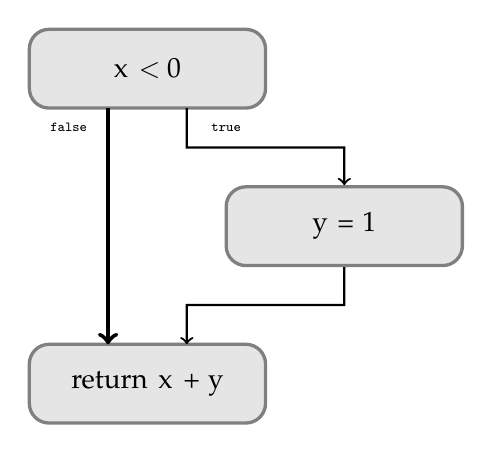
\begin{tikzpicture}[
    graynode/.style={
      rectangle, 
      draw=gray!100, 
      fill=gray!20.5, 
      very thick, 
      minimum size=5mm,
      minimum height=1cm,
      minimum width=3cm,
      rounded corners=0.25cm
    }
    ]
    \node[graynode] (l1) at (0,4cm) {\lstinline{x < 0}};
    \node at (1,3.25) {\tiny${\tt true}$};
    \node at (-1,3.25) {\tiny${\tt false}$};
    \node[graynode] (l2) at (2.5cm,2cm) {\lstinline{y = 1}};
    \node[graynode] (l3) at (0,0) {\lstinline{return x + y}};
    \draw[thick,->] (l1)++(0.5,-0.5) -- (0.5,3) -- (2.5,3) -- (l2);
    \draw[thick,->] (l2) -- (2.5,1) -- (0.5,1) -- (0.5,0.5);
    \draw[ultra thick,->] (-0.5,3.5) -- (-0.5,0.5);
  \end{tikzpicture}
\caption{Control-Flow Graph for function \lstinline{f()}.  On the bold path, \lstinline{y} is undefined.}
\label{f:c8_cfg_1}
\end{figure}

\subsection{Loops}

The treatment of loops with respect to definite assignment warrants special attention.  Recall the mechanism for determining definite assignment is conservative.  In the context of loops, it simply assumes {\em every loop can be executed zero or more times} (i.e. even if this is not correct).  The following illustrates:

\begin{lstlisting}
function f(int x) -> int:
   int y
   //
   while x < 0:
       y = 1
       x = x + 1
   //
   return x + y
\end{lstlisting}

The above function fails definite assignment because variable \lstinline{y} is not defined when zero iterations of the loop are executed (e.g. when \lstinline{x==0} on entry).  To illustrate the conservative nature of definite assignment, consider this variation:

\begin{lstlisting}
function ten() -> int:
   int x = 0
   int y
   //
   while x < 10:
       y = 1
       x = x + 1
   //
   return y
\end{lstlisting}

Here, it can be shown that \lstinline{y==1} must hold when the \lstinline{return} statement is reached.  Nevertheless, this function fails definite assignment because of the assumption that the loop executes {\em zero} or more iterations.

\subsection{Infeasible Paths}

Functions and methods may contain \glslink{infeasible_path}{infeasible paths} which are valid execution paths that, in practice, cannot be executed.  The mechanism for checking definite assignment assumes for simplicity that any valid path can be executed.  This means that some programs will fail definite assignment, even though they can be shown as safe.   The following illustrates such a program:

\begin{lstlisting}
function abs(int x) -> int:
    int y
    //
    if x >= 0:
        y = x
    //
    if x < 0:
        y = -x
    //
    return y
\end{lstlisting}

This function contains four valid execution paths which can be denoted by \lstinline{ff}, \lstinline{tf}, \lstinline{ft}, \lstinline{tt} where, for example, \lstinline{tf} represents the path where the first condition evaluates to \lstinline{true} and the second to \lstinline{false}.  However, it is easy to see that execution paths \lstinline{ff} and \lstinline{tt} are infeasible.  Furthermore, that on the other two paths, \lstinline{tf} and \lstinline{ft}, variable \lstinline{y} is definitely assigned at the \lstinline{return} statement.  Despite this, the above function fails definite assignment because the mechanism considers all valid paths whilst ignoring infeasible execution paths.

\subsection{Partial Assignments}

A variable will never be considered definitely assigned after the application of one or more {\em partial assignments}.  The following illustrates a program which fails definite assignment even though it can be shown as safe:

\begin{lstlisting}
type Point is {int x, int y}

function Point(int x, int y) -> Point:
    Point p
    p.x = x
    p.y = y
    return p
\end{lstlisting}

In the above program, the variable \lstinline{p} can be shown as definitely assigned at the \lstinline{return} statement.  Nevertheless, the conservative mechanism for checking definite assignment will reject this program because variable \lstinline{p} is initialised via partial assignments.  

\section{Description}

Definite assignment is defined over the \gls{control_flow_graph} of a code block, such as a \lstinline{requires} or \lstinline{ensures} clause, or the body of a function or method.  Appendix~\S\ref{c_cfg} details the process for constructing a control-flow graph from a block of code.  

Definite assignment considers the set of all {\em valid paths} in a \gls{control_flow_graph}.  A valid path is a path through the graph starting from its root.  Every vertex in the graph is associated with a set of variables which are {\em defined} at that vertex, as well as those which are {\em used} at that vertex.  A variable $x$ is said to be {\em definitely assigned} on entry to a vertex $v$ if, for every valid path which includes $v$, some ancestor vertex $u$ exists on which $x$ is defined.

\subsection{Definitions and Uses}

A \gls{variable_definition} occurs at a vertex $v$ which contains a direct assignment (recall~\S\ref{c_stmt_assign}), or an initialisation of (recall~\S\ref{c_stmts_var_decl}), one or more variables.  Assignments to fields, array elements or dereferenced references are not direct and do not define variables.  A vertex may define multiple variables if it corresponds to a multiple assignment which directly assigns those variables.  Finally, the parameters of a function, method or invariant block are treated as being defined on entry. 

A \gls{variable_use} occurs at a vertex $v$ which directly refers to that variable in some expression other than an \lstinline{LVal}.  However, referring to a variable indirectly through a dereference expression does not constitute a variable use.

%\section{Verification}

As discussed in the introduction, an important feature of Whiley is
{\em verification}.  That is made up of two aspects: firstly, the
ability to write specifications for functions and methods in Whiley;
secondly, the ability of the compiler to check the body of a function
or method meets its specification.

Unfortunately, specifications is not always straightforward and
requires considerable attention to detail.  Nevertheless, with
practice, it can easily fit into the routine of day-to-day
development.  In this section, we'll explore the basics of
verification in Whiley and, in the following section, we'll look at
practical example.

\paragraph{Example.}  To illustrate verification in Whiley, we'll
consider specifying a simple example function.  This is the
\lstinline{contains()} function, described as follows:

\begin{lstlisting}
// Returns true if the items list contains the given item and false otherwise.
function contains([int] items, int item) => bool:
    ...
\end{lstlisting}

This is a common function found in the standard libraries of many
programming languages.  The body of the function examines each element
of the \lstinline{items} list and check whether or not it equals
\lstinline{item}.  To start with, we won't worry too much about the
body of the \lstinline{contains()} function.  Instead, we'll
progressively build up the specification until we are happy with it.
Then, we'll give an implementation of the function which meets this
specification.



\chapter{Error Messages}

{\bf Note:} need to distinguish the different kinds of error; e.g. type errors versus other errors?

\section{Parse Errors}

\section{Declarations}

\subsection{``Cyclic Constant Declaration'' (301)}

A {\em cyclic constant declaration} occurs when a \gls{constant_declaration} refers to itself, either {\em directly} or {\em indirectly}.  This is an error because constants must be evaluated at \gls{compile_time}.

\paragraph{Example.}  The following illustrates several cyclic constant declarations:

\begin{lstlisting}
constant const1 is 1 + const1

constant const2 is 1 + const3
constant const3 is 1 + const2
\end{lstlisting}
Here, all three constant declarations are cyclic.  The declaration for \lstinline{const1} has a {\em direct} cycle, because its definition refers to itself.  The declaration for \lstinline{const2} has an indirect cycle, because its definition refers to \lstinline{const3} which, in turn, refers back to \lstinline{const2}.

\section{Expressions}

%\subsection{``Invalid File Access'' (000)}

%\subsection{``Invalid Package Access'' (000)}

%\subsection{``Resolution Error'' (000)}

\subsection{``Variable Possibly Uninitialised'' (000)}
\label{c_err_var_uninitialised}
A {\em variable possibly uninitialised} occurs when a variable may be used without being defined.  That is, when a simple path exists through the control-flow graph of a function or method from that variable's declaration to a use which contains no definition for that variable.  This error is reported as part of the {\em definite assignment} checking performed during compilation (see~\S\ref{c_definite_assignment}).

\paragraph{Example.}  The following illustrates a variable which is possibly uninitialised:

\begin{lstlisting}
function f(int x) => int:
   int y
   return x + y
\end{lstlisting}

Here, variable \lstinline{y} is definitely uninitialised in the expression ``\lstinline{x + y}''.  For more examples of variables which are possibly uninitialised, see~\S\ref{c_definite_assignment}.

\subsection{``Ambiguous Coercion'' (000)}

An {\em ambiguous coercion} occurs when the target of a cast expression is uncertain.  That is, when attempting to cast a value to a given type \lstinline{T}, but there is more than one way this can be achieved.  This error is reported as part of the {\em coercion check} performed during compilation.

\paragraph{Example.}  The following illustrates an ambiguous coercion:

\begin{lstlisting}
type Ambiguous is { int f1, real f2} | { real f1, int f2 }

function f(int x, int y) -> Ambiguous:
   return (Ammbiguous) {f1: x, f2: y}
\end{lstlisting}

The cast is ambiguous here because it's unclear whether, for example, \lstinline|{f1: 1, f2: 2}| should become \lstinline|{f1: 1.0, f2: 2}| or \lstinline|{f1: 1, f2: 2.0}|.

\section{Control Flow}

\subsection{``Invalid LVal'' (000)}

An {\em invalid lval} error occurs when an invalid expression is used on the left-hand side of an assignment.  Only expressions which are also lval's maybe used in such a situation  (see~\S\ref{c_stmts_lval}).

\paragraph{Example.}  The following illustrates two invalid lval's:

\begin{lstlisting}
function f(int x):
   1 = x   // constant not valid lval
   x+1 = x // arithmetic expression not valid    
\end{lstlisting}

The first assignment statement is invalid because one cannot assign to a constant.  The second is invalid because one cannot assign to an arithmetic expression.

\subsection{``Invalid Destructuring LVal'' (000)}

An {\em invalid destructuring lval} occurs when a destructuring assignment is used on the left-hand side, but the right-hand side returns an incorrect number of values.

\paragraph{Example.}  The following illustrates an invalid destructuring LVal:

\begin{lstlisting}
function f(int x, int y) -> int:
    return x+y

function g(int x, int y) -> int:
    x,y = f(x,y)
    return x - y
\end{lstlisting}

Here, the invocation of \lstinline{f()} in \lstinline{g()} uses an invalid destructuring assignment because \lstinline{f()} returns one value, the assignment expects two.

\subsection{``Break Outside of Loop'' (000)}

A {\em break outside loop} occurs when a \lstinline{break} statement is given which is not contained within one or more loops.  This is an error because the break statement is used specifically to exit a loop early, and must be contained within the loop to be exited.  

\paragraph{Example.}  The following illustrates a break outside of a loop:

\begin{lstlisting}
function f(int x) -> int:
   break
   return x
\end{lstlisting}

Here, the \lstinline{break} statement is meaningless as it is not associated with a loop.

\subsection{``Unknown Variable'' (000)}

An {\em unknown variable} occurs when an attempt is made to access a variable which has not been declared in the current scope.  All variables must be declared before they can be used.

\paragraph{Example.}  The following illustrates an unknown variable:

\begin{lstlisting}
function f(int x) -> int:
   return x+y
\end{lstlisting}

Here, the \lstinline{return} statements refers to an unknown variable \lstinline{y}.  In contrast, the reference to variable \lstinline{x} is valid because \lstinline{x} has been declared within scope.

\subsection{``Unknown Function or Method'' (000)}

\subsection{``Variable Already Defined'' (000)}

A {\em variable redefinition} occurs when a variable is declared with a name matching another variable already in scope.  This is an error because it is not permitted for one variable to shadow another.

\paragraph{Example.}  The following illustrates an example of a variable redefinition:

\begin{lstlisting}
function add([int] xs, int v) => [int]:
    for k,v in xs:
        xs[k] = xs[k] + v
    return xs
\end{lstlisting}

Here, the \lstinline{for} loop attempts to declare a variable \lstinline{v}, but another variable \lstinline{v} was already declared as a parameter.

\subsection{``Duplicate Default Label'' (000)}
A {\em duplicate default label} occurs when a \lstinline{switch} statement includes more than one \lstinline{default} label.  This is an error because at most one \lstinline{default} is permitted.

\paragraph{Example.}  The following illustrates an example of a duplicate \lstinline{default} label:

\begin{lstlisting}
function f(int x):
    switch x:
        case 0:
            return 0
        default:
            return 1
        default:
            return 2
\end{lstlisting}

Here, the \lstinline{switch} statement has two \lstinline{default} labels.  This must be an error as, otherwise, it would be ambiguous as to which executed.

\subsection{``Duplicate Case Label'' (000)}
A {\em duplicate case label} occurs when a \lstinline{switch} statement includes more than one \lstinline{case} label matching the same value.  This is an error because at most one \lstinline{case} matching a given value is permitted.

\paragraph{Example.}  The following illustrates an example of a duplicate \lstinline{case} label:

\begin{lstlisting}
function f(int x):
    switch x:
        case 0:
            return 0
        case 0,1:
            return 1
        default:
            return 2
\end{lstlisting}

Here, the \lstinline{switch} statement has two \lstinline{case} labels, both of which match the value \lstinline{0}.  This must be an error as, otherwise, it would be ambiguous as to which executed.

\subsection{``Unreachable Code'' (000)}

In a function or method, {\em unreachable code} arises when no possible execution path could reach them.  

\paragraph{Example.} The following illustrates some unreachable code:

\begin{lstlisting}
function abs(int x):
    //
    if x < 0:
        return -x
    else:
        return x
    //
    return 0 // unreachable
\end{lstlisting}

Here, the final \lstinline{return} statement can never be reached by any execution path through the \lstinline{abs()} function.  This is considered an error because it indicates something undesirable which may not have been intended.

\subsection{``Missing Return Value'' (000)}

\subsection{``Branch Always Taken'' (000)}

\section{Functions (000)}

\subsection{``Reference Not Permitted in Function'' (000)}

\subsection{``Method Invocation Not Permitted In Function'' (000)}

\subsection{``Reference Access Not Permitted in Function'' (000)}

\subsection{``Return from Void'' (000)}
	
\section{Types (000)}

\subsection{``Subtype Error'' (000)}

\subsection{``Incomparable Operands'' (000)}

\subsection{``Record Type Required'' (000)}

\subsection{``Record Missing Field'' (000)}



%\input{regions}
%\input{finiteness}
%\section{Foreign Function Interface}
\label{s_ffi}
The {\em Foreign Function Interface (FFI)} provides a mechanism to enable code written in Whiley to interact with code written in another programming language.  In this section, we will discuss those mechanisms provided in Whiley for this purpose.  Of course, the Whiley system cannot make any guarantees about such external code and care must be taken to ensure it treats types and specifications correctly.  

\subsection{Overview}

The foreign function interface represents a boundary between internal (i.e. Whiley) code and external code written in other (i.e. {\em foreign}) languages.  Whiley provides two modifiers for functions and methods which allow information to flow across this boundary.  These are:

\begin{itemize}
\item The \lstinline{native} modifier, which declares a function or method which is {\em implemented} in a foreign language.  That is, a function or method whose implementation is written in another language.  Code written in Whiley can call this function, and the compiler is responsible for correctly routing this to the actual function body.

\item The \lstinline{export} modifier, which declares a function or method that is {\em visible} to foreign code.  That is, a function or method which may be called from foreign code.  This provides a way for foreign code to invoke Whiley function and methods.
\end{itemize}

These modifiers provide two different mechanisms for allowing information to flow between code written in Whiley and code written in a foreign language.  As an example, recall the Minesweeper example from \S\ref{s_minesweeper}.  Suppose we wanted to implement a Graphical User Interface for our minesweeper game in Java.  There are two ways we could approach this:

\begin{itemize}
\item {\bf Whiley as ``Master''}.  In this case, the Whiley code is considered the primary implementation and provides the entry point to the application.  In contrast, the Java code is consider subservient and is always called from Whiley.
\item {\bf Whiley as ``Slave''}.  In this case, things are the other way around.  The Java code is considered the primary implementation and provides the application's entry point.  The Whiley code, on the other hand, simply provides supporting functions and methods for this.
\end{itemize}

For this particular situation, it probably makes most sense to follow the ``Whiley as Slave'' approach.  This makes sense if we view our completed Minesweeper game as an instance of the {\em Model-View-Controller (MVC)} pattern.  According to this, the Whiley implementation of Minesweeper illustrated in \S\ref{s_minesweeper} corresponds to the {\em model}.  The Graphical User Interface would then correspond to the {\em view}.

% \subsection{Example: Whiley as Master}

% \subsection{Example: Whiley as Slave}

% call this function from code written in the Java programming language.  To do this, we need to declare this function using the \lstinline{export} modifier:

% \begin{lstlisting}
% // Return the square on a given board at a given position
% export function getSquare(Board b, int col, int row) => Square:
%     ...
% \end{lstlisting}

% Here, the \lstinline{export} modifier declares that \lstinline{getSquare()} may be called from foreign code.  Furthermore, suppose we have declared \lstinline{getSquare()} in the file \lstinline{Minesweeper}.  Then, the following Java code can be used to call this function:



\printglossaries

\bibliographystyle{unsrt}
\bibliography{abbrevs,references}

\end{document}
